\documentclass[12pt,a4paper]{article}
\usepackage{times}
\usepackage{durhampaper}
\usepackage{harvard}
\usepackage{graphicx}
\usepackage{algpseudocode}
\usepackage{algorithm}
\usepackage{subcaption}
\usepackage{caption}
\renewcommand{\harvardurl}{URL:\url}
\citationmode{abbr}
\bibliographystyle{agsm}

\title{User Interaction Discovery in Virtual Environments}
\student{L. A. Sutton}
\supervisor{W. Li}
\degree{BSc. Natural Sciences}

\date{\today}

\begin{document}

\maketitle

\begin{abstract}

{\bf Context/Background}
Within the past 20 years there has been an explosion in computer mediated interactions between people. There has been much previous work in the area of visualising networks of people in these virtual environments such as social networks or within office communication systems, however this has almost exclusively focused on static systems of relationships rather than a representation of the dynamic interactions themselves.

{\bf Aims}
What has been learned from the visualisation of static networks of relationships will be applied to the representation of dynamic systems with a focus on the interactions between the users rather than simple the static relationships in order to produce a new visualisation system that will allow new features of data sets to become apparent.

{\bf Method}
A system has been created in Python using the Pygame library to represent various different modes of interactions between users in a virtual environment in different ways along with the state of the users. This system has then been applied to various models of real-world scenarios in order to demonstrate its utility.

{\bf Results}
The system is able to effectively represent several different real-world scenarios across a wide variety of situations for example the spread of viral advertising, the propagation adoption of certain behaviours or a trust-based recommendation system. Furthermore it can be seen that this system of looking at interactions is more effective than currently available approaches in several areas. This is shown by the visual output that my solution has produced which effectively represent the situations listed above in ways clearer than would otherwise be possible.

{\bf Conclusions}
In conclusion the results of this solution meet the aims given above. The application to various models show how my solution is able to represent systems in terms of the interactions between users and how these interactions evolve over time. Additionally they show how this is a more useful way of looking at these systems that simply a static graph of relationships.

\end{abstract}

\begin{keywords}
user interaction; virtual environments; visualisation; clustering
\end{keywords}

\section{Introduction}

\noindent   
In the 21st century, people spend more time than ever interacting in virtual environments. Figure \ref{fig:interactions} shows how social media and email in particular are not only very commonly used in the UK, but still growing in popularity. With this growth it is clear that it is becoming ever more important that these systems of relationships and interactions can be better understood not only though statistical analysis, but through effective visualisation.

There is a long history of visualising the structures that form within these environments \cite{freeman2000visualizing}. This has evolved significantly over time with early graphs of relationships being hand drawn to the present day where layout algorithms running on computers make it possible to visualise ever more complex graphs with greater numbers of nodes effectively. 

Finally, as an extension of these graphs, interactivity has become possible such that they are able to be manipulated in real time. This then allows increasingly novel ways of visualising data and opens up the possibility that these graphs can be used to show more than simply static relationships but rather become effective tools for visualising a dynamic system of interactions that evolves over time.

\begin{figure}[htb]
\centering
\caption{Graph of growth on online interactions in the UK \protect\cite{ons}}
\label{fig:interactions}
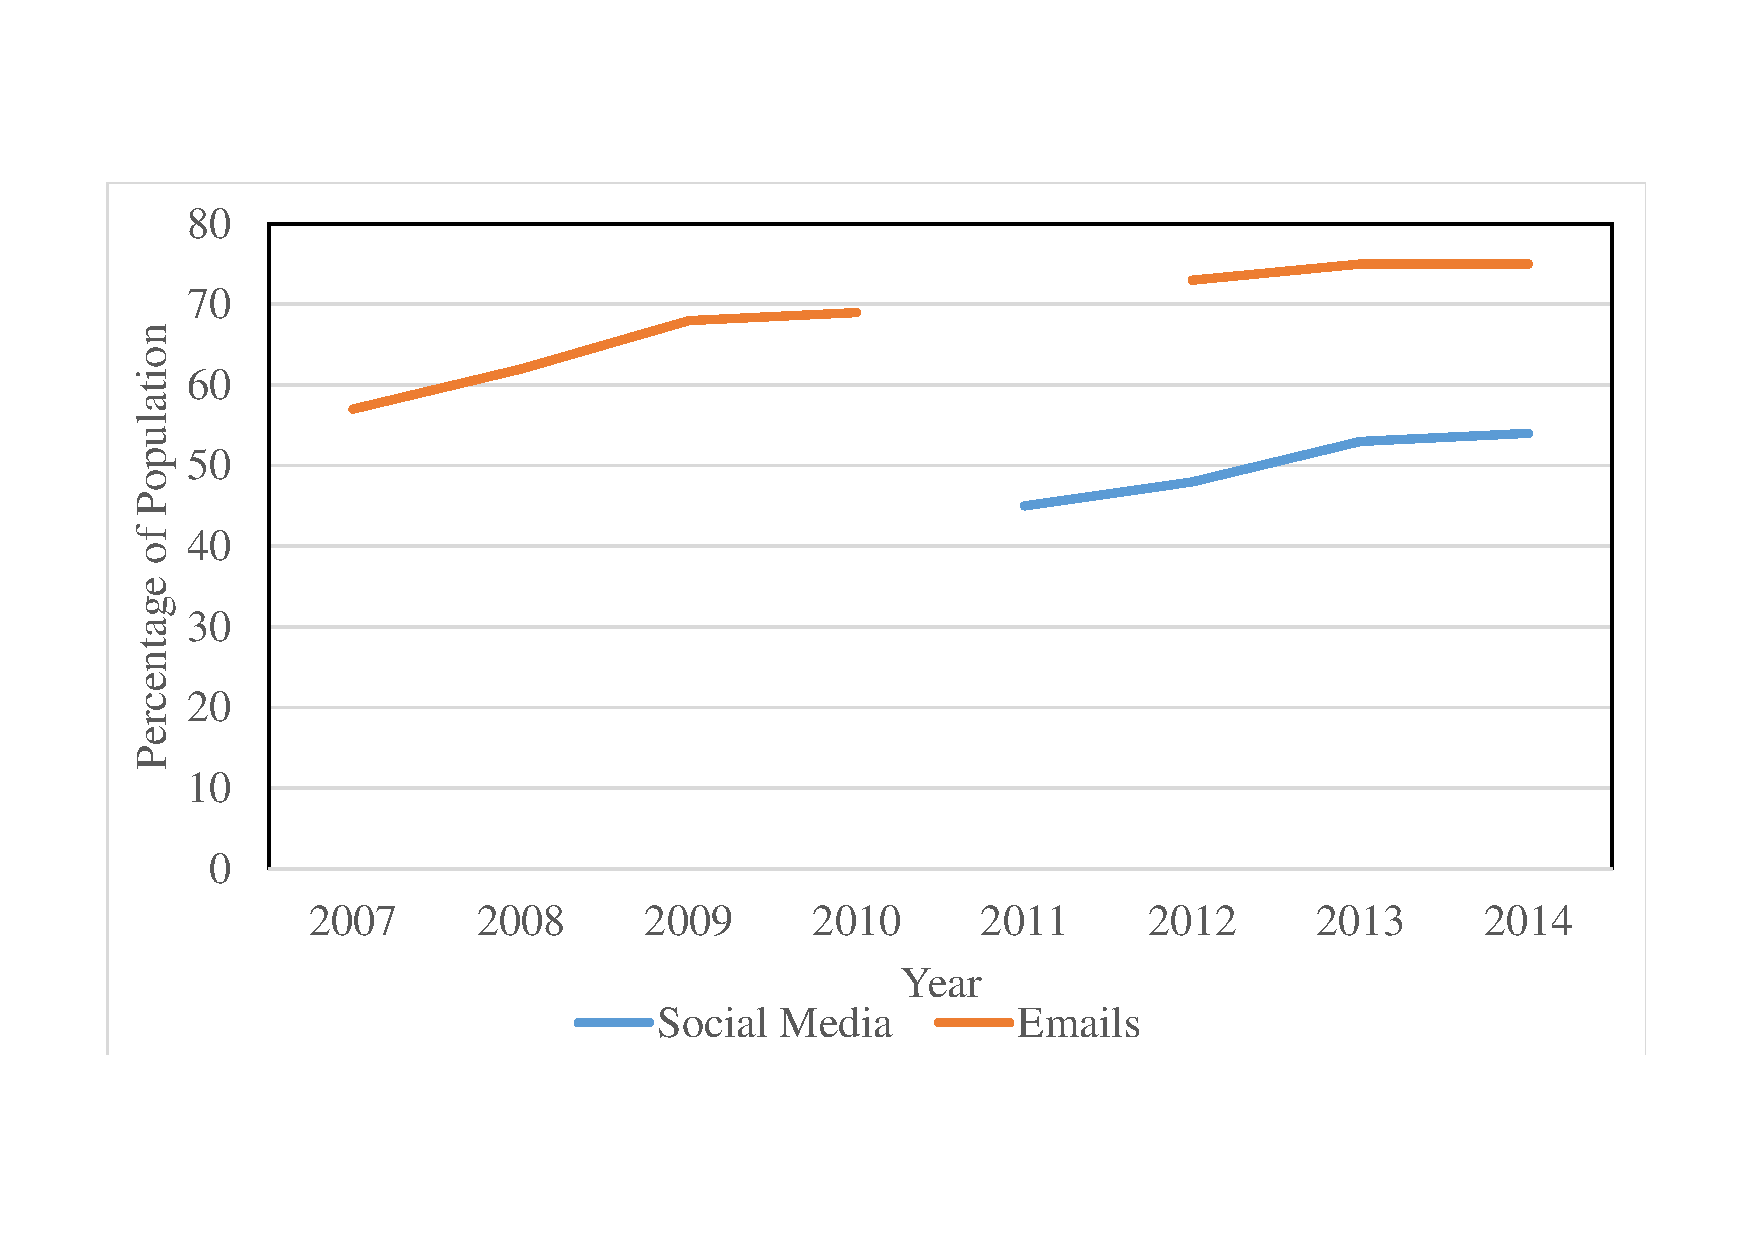
\includegraphics[scale=0.4]{Chart.pdf}
\end{figure}

In this project I have taken 'User Interaction' to mean any way in which users consciously affect other users so that the other users would be able to identify the specific other users they were interacting with. This could take place over a period of time of be instantaneous; it could be between two users or many; it could be a single event or it could be ongoing. For example I will consider interactions such as users sending emails between one another but I will not consider interactions such as a user's advertising preference changing what another user sees as this falls beyond my scope.

Virtual environments in this project will mean any environment in which users are able to interact in the ways I have previously mentioned, mediated by computers. This will most likely mean over the internet, however it could also be the case that it occurs over smaller network such as within an office or university internal network. This could be for example a video game, a social networking website or a messaging system such as email.

\subsection{Project Motivation}

While there have been many previous attempts to visualise the structure of virtual environments, these have have two drawbacks. Firstly they have only bee interested in static 'snapshots' of social networks that either represent their state at a particular time or assume that they do not change significantly over time. This is no surprise as the ability to produce dynamic representations is a relatively new ability in the long history or social network representation. Secondly they have focused only on the relationships between people within these networks rather than exploring other aspects of the system at a more fundamental level.

With increasing ease of interacting in virtual environments and the explosion in modes over which these interactions are possible it is increasingly important that new ways are developed to visualise this data. It was therefore decided that the current systems could be extended in two ways.

Firstly I wanted to extend the existing work that covered these static representations of relationships and take what was learned to apply to dynamic systems of interactions that were able to evolve over time.

Secondly I wanted to move the focus of the systems away from the current system of representing only the relationships between users that are inferred from the interactions. I would instead represent the interactions themselves.

\subsection{Project Aims}

These are the aims for the project, as laid out in the Design Report.

\begin{enumerate}
\item Basic Deliverables
\begin{enumerate}
\item Develop a simple system that models user interactions with a visual output
\item Use this system to implement an existing model of user interaction
\item Expand this system and model to be able to visualise different modes of interaction
\end{enumerate}
\item Intermediate Deliverables
\begin{enumerate}
\item Expand the initial system so that its state will evolve over time according to the interactions of its users
\item Examine and visualise the way in which users cluster according to their interactions
\item Allow the system to set its initial state by real-world social network data
\end{enumerate}
\item Advanced Deliverables
\begin{enumerate}
\item Visualise change in the clustering of users according to their interactions over time
\item Generate quantitative output related to the change in clustering of users over time
\item Apply my quantitative output to attempt to solve a real-world problem
\end{enumerate}
\end{enumerate}

\section{Related Work}

\subsection{Social Network Visualisation}
As I have already mentioned, network visualisation is a science with a long history, the interest here however is after computer started being used to assist in the drawing of graphs. There are currently low-level tools that exist with the intention that they have the necessary flexibility to accommodate a wide variety of visualisation styles and techniques \cite{heer2005prefuse}. As well as this, there are tools that exist to provide numerical analysis \cite{borgatti2002ucinet}. However, these tools have focused on the analysis and visualisation of snapshots of data remaining static, rather than data sets that evolve over time. They therefore demonstrate the problems that I have talked about above. These have also previously been used to build ways of visualising social network data from Friendster \cite{heer2005vizster} in order to facilitate discovery of more information than would be apparent from other ways, showing that there is merit in using a graphical approach, and indicating that another approach may be useful.

\subsection{Information Presentation}
There is also a wide variety of information on the presentation of data on computer screens.The most popular model can be summed up as 'Overview, Zoom, Filter' \cite{shneiderman1996eyes}. In this model it is suggested that the initial view of the data should be a movable field of view with emphasis on allowing the user to gain an 'overview' of relevant data and identify areas which will be of interest. Specific areas of interest can then be zoomed in on preserving the context of the overall picture before extra information of areas of interest can be viewed possibly by clicking on them. This paper also talks about the importance of smooth display updates and responsiveness to user input, something also considered in this project. This is built upon by the ideas of making information more clear by distorting the 'presentation space' \cite{carpendale2001framework}. This is the method used in Vizster and can be seen in common usage in many different data visualisation applications. It imagines that the virtual space in which the data is presented is a real material that can be stretched and viewed through a movable lens as necessary to make the relevant areas of the information more clear. These ideas area also expanded on further to see what kinds of lenses are suitable for which purposes, and mathematical frameworks for implementing such a lens \cite{leung1994review} have been discussed. Together these papers can provide a unified way of presenting graphs in a dynamic way by as the techniques are complimentary. This is the approach that will therefore be taken in this project.

\subsection{Graph Drawing}
There is also previous literature on the drawing of graphs in aesthetically pleasing ways. Almost all current research makes use of a force directed spring layout. In this algorithm, each node is modelled is repelling each other node and the edges between them are modelled as springs\cite{fruchterman1991graph}. Included in these papers are suggestions for the strength of the attractive and repulsive forces different distances and the size of graph that this can be expected to create. However, this algorithm doesn't scale well with rapidly increasing numbers of vertices. It has been pointed out that with a large number of nodes, calculating the layout in this way is very expensive in terms of computing power. However, with the correct optimisations it is possible to reduce the complexity to $o(nlog(n))$ \cite{barnes1986hierarchical}. However, this significantly increases the complexity of the implementation. A compromise is therefore taken in this solution whereby there is a limit on the number of nodes that can be laid out for a given application.

\subsection{Modelling Network Interactions}
The ability to produce networks of relations and interactions from many different data sources is also explored in a variety of different papers. For example, networks of social interaction have been produced from a history of email correspondence within an organisation \cite{fisher2004social} or the transcript of an internet relay chat \cite{mutton2004inferring}. It is also possible to use data gathered from a users's social network using tools made for the purpose of downloading such data in a usable form. For example Netvizz (https://apps.facebook.com/netvizz/)
%Here other relevant ideas are explored such as the privacy implications of collecting data on a large scale and the ability to reconstruct the whole graph from only partial data. The same has also been achieved using the transcript of an internet relay chat \cite{mutton2004inferring} again struggling with the problem of reconstructing a complete graph from partial data. It is then further shown that the same method including the temporal decay of relationships can be applied to other sources of relationship information involving over time such as the plays of William Shakespeare.
There are also many models that have been proposed for interactions in other ways. These include models for the spread of influence \cite{kempe2003maximizing}, the spread of viral advertising \cite{van2010viral} and a proposal for a social recommendation system \cite{walter2008model}. The combination of all of these gives many possible systems which can be used to demonstrate the effectiveness of the system.

\subsection{Categorisation of Interactions}
Previous research has also explored categorisation of interactions by their characteristics. This has mainly in the past been applied to social iterations within 3D virtual environments in which people interact as virtual avatars, referred to as Networked-Virtual Environments. One particular application of this is games \cite{manninen2000interaction}. Here we can see that there is more than one way of categorising interactions, one way being based on their purpose. These papers also show how it is possible for many different modes of interaction to happen simultaneously. It is possible to use communicative action theory to categorise interactions by their purpose, this is extended in other papers by comparing interactions in a selection of game environments \cite{becker2002social}. Extending this to other environments such as the social network, other papers show how much of the interaction that goes on writhing a virtual environment is hidden from the user. We can see just how much data website such as Facebook collect about us including in our making interactions which we wouldn't normally consider meaningful \cite{schneier2010taxonomy}

%\subsection{Evolution of social networks}
%Ideas of the behaviour of users in social networks have been the subject of many different papers. This includes homophily \cite{adamic2003social} which is the idea that people on social networks tend to associate with people who are similar to themselves in terms of age, political views etc. Work has also been completed on the behaviours of users within a social network and the ways in which interactions can spread behaviour across networks of people represented as graphs. It has been suggested that this can be explained using a virus like model \cite{centola2010spread} in which users pass between susceptible, infected and recovered states, analogous to a computer-virus or a real virus.

\subsection{Detection of clustering}
Detecting features of social networks that are not immediately apparent is also extremely important. We can see that algorithms have been developed that aim to detect communities, related to clustered sections of graph representations of these networks \cite{newman2004fast}. These algorithms can be applied to real world networks with a good degree of success reported in identifying the same communities that the users themselves identify with. Given the visual nature of my project I will therefore endeavour to present the graph in such a way that any clustering based on interactions between the users becomes obvious.

\section{Solution}

My solution focuses on flexibility and allows the user to enable and disable as well as configure many different elements. These various elements are described below.

\begin{figure}[htb]
\centering
\caption{Architectural diagram of solution}
\label{fig:diagram}
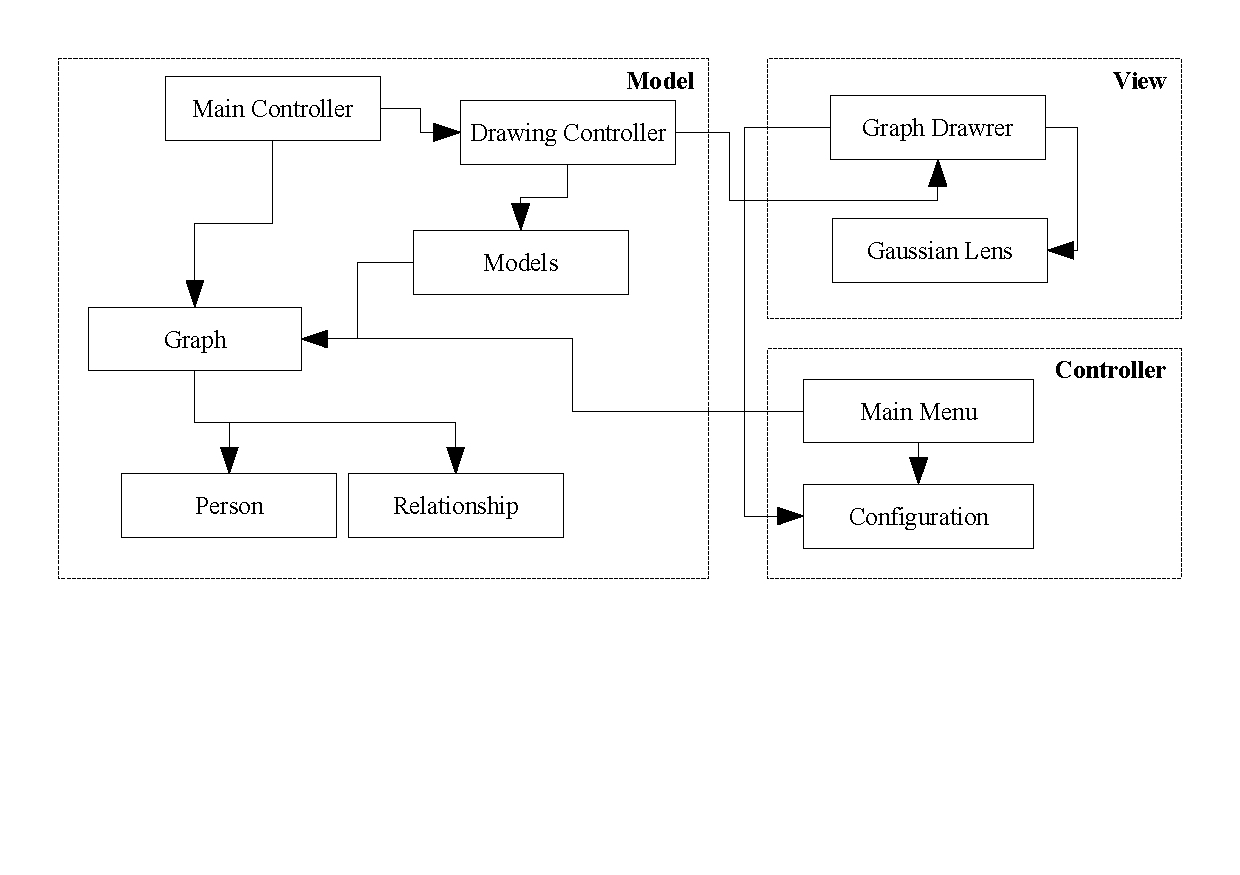
\includegraphics[scale=0.75]{ArchitectureDiagram.pdf}
\end{figure}

As was described in my Design Report, I have used a 'Model, View, Controller' software pattern to guide the architecture of my solution. This has allowed the compoenets to remain as separate as possible as shown in figure \ref{fig:diagram}.

It can be seen in this diagram how the the Model contains all necessary logic in the system along its state with the Drawing Controller and the Graph while keeping this separate from the Controller which handles the Menu generation and storage of its results. The View is then again separate and can focus on its interactions with the Model and the Controller to draw the graph and distort it with the Gaussian Lens.

\subsection{Menu System}

The primary control of the system is given initially though a system of menus which are presented to the user before the system begins running.

\begin{figure}[htb]
\centering
\caption{Example menu system of the solution}
\label{fig:menu}
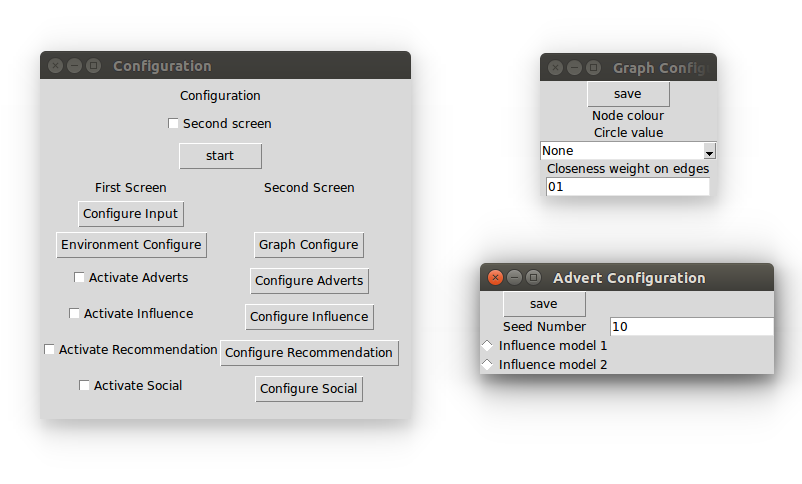
\includegraphics[scale=0.5]{MenuShot.png}
\end{figure}

Figure \ref{fig:menu} shows an example of these menus. The main window on the left represents the main control of the application. In this window it is possible to enable and disable various models that can be used in order to demonstrate the visualisation system. The buttons next to these check boxes allow various aspects of each the demonstration to be configured so as to give different results. The aspects that can be configured are detailed in the descriptions of each system below.

This menu also allows the user to select what initial input data will be used. They can either generate random data that will be realistic enough in order to demonstrate the system or import their own data. Users own data will come from the netvizz Facebook app (https://apps.facebook.com/netvizz). This allows users to download a '.gml' file containing a list of all friends of a user, the sex of the users, how many things they like and a separate list of all friendships between the listed users in order to build up a network.

\subsection{Interactions with Vertices}

The user is able to interact with vertices representing people in the graph in two different ways. These are shown in \ref{fig:labels}.

\begin{figure}[htb]
\centering
\caption{Diagram showing labels and selctions}
\label{fig:labels}
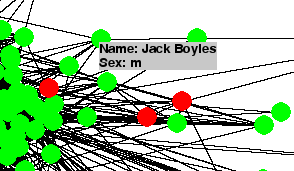
\includegraphics[scale=1]{Select.png}
\end{figure}

The first way is that if the user has selected it as an option in the first menu, they have the ability to move their mouse over a node in order to see more information about it. This can be seen as the box with a grey background in the figure. It can be configured to show what information the user requests, in this case it shows the name and sex of the person represented by the vertex.

The second way in which the user can interact directly with vertices is by clicking on them. This has a different meaning depending on the context for example, it could be used to select the points being used to seed in the advert or influence models laid out below, the colour change is then used to indicate which vertices are selected.

\subsection{Graph Layout}

This element of my solution is always enabled and allows the system to lay out the graph which forms the basis for for its representation of interactions. The system that I have used to lay out my graph is based on a previous sprint-directed layout algorithm \cite{fruchterman1991graph}.

Current data visualisations make almost exclusive use of a force-directed spring layout for graph drawing. This method models a graph as a set of springs along each edge joined at each node. These springs, as in my case, need not respond to force in the same way as a real, physical spring but can instead have whatever response gives the best layout for the graph.

The algorithm can then use an iterative approach in order to find a local point of least tension on the springs as a collection. 

\begin{algorithm}[htb]
\caption{Graph sprint-directed layout algorithm}
\label{alg:graph}
\begin{algorithmic}
\State $graph \gets (V, E)$ \Comment{Graph represented as a collection of vertices and edges}
\State $k \gets \sqrt{1/|V|}$
\State $t \gets 0.05$
\ForAll{Vertex in V}
	\State $Vertex.displacement \gets (0,0)$
	\ForAll{Other in V \textbackslash Vertex}
		\State $dist \gets distance(Vertex, Other)$ \Comment{$distance$ gets Euclidean distance}
		\State $diff \gets (Vertex.x-Other.x, Vertex.y-Other.y)$
		\State $Vertex.displacement \gets Vertex.displacement + diff \times (k^{2}/dist)$
	\EndFor
\EndFor
\ForAll{Edge in E} \Comment{Edge between two vertices, $V_{1}$ and $V_{2}$}
	\State $dist \gets distance(V_{1}, V_{2})$
	\State $diff \gets (V_{1}.x-V_{2}.x, V_{1}.y-V_{2}.y)$
	\State $V_{0}.displacement \gets V_{0}.displacement - diff \times (dist^{2}/2k)$
	\State $V_{1}.displacement \gets V_{1}.displacement + diff \times (dist^{2}/2k)$
\EndFor
\ForAll{Vertex in V}
	\State $(Vertex.x, Vertex.y) \gets (Vertex.x, Vertex.y) + (Vertex.displacement/distance(Vertex.displacement)) \times (min(distance(Vertex.displacement), t))$ \Comment{$min$ gives minimum of two elements}
	\State $(Vertex.x, Vertex.y) \gets min(0.95, max((Vertex.x, Vertex.y), 0.05))$ \Comment{$max$ gives maximum of two elements}
\EndFor
\end{algorithmic}
\end{algorithm}

\begin{figure}[htb]
\caption{Graph Layout}
\label{fig:layout}
\centering
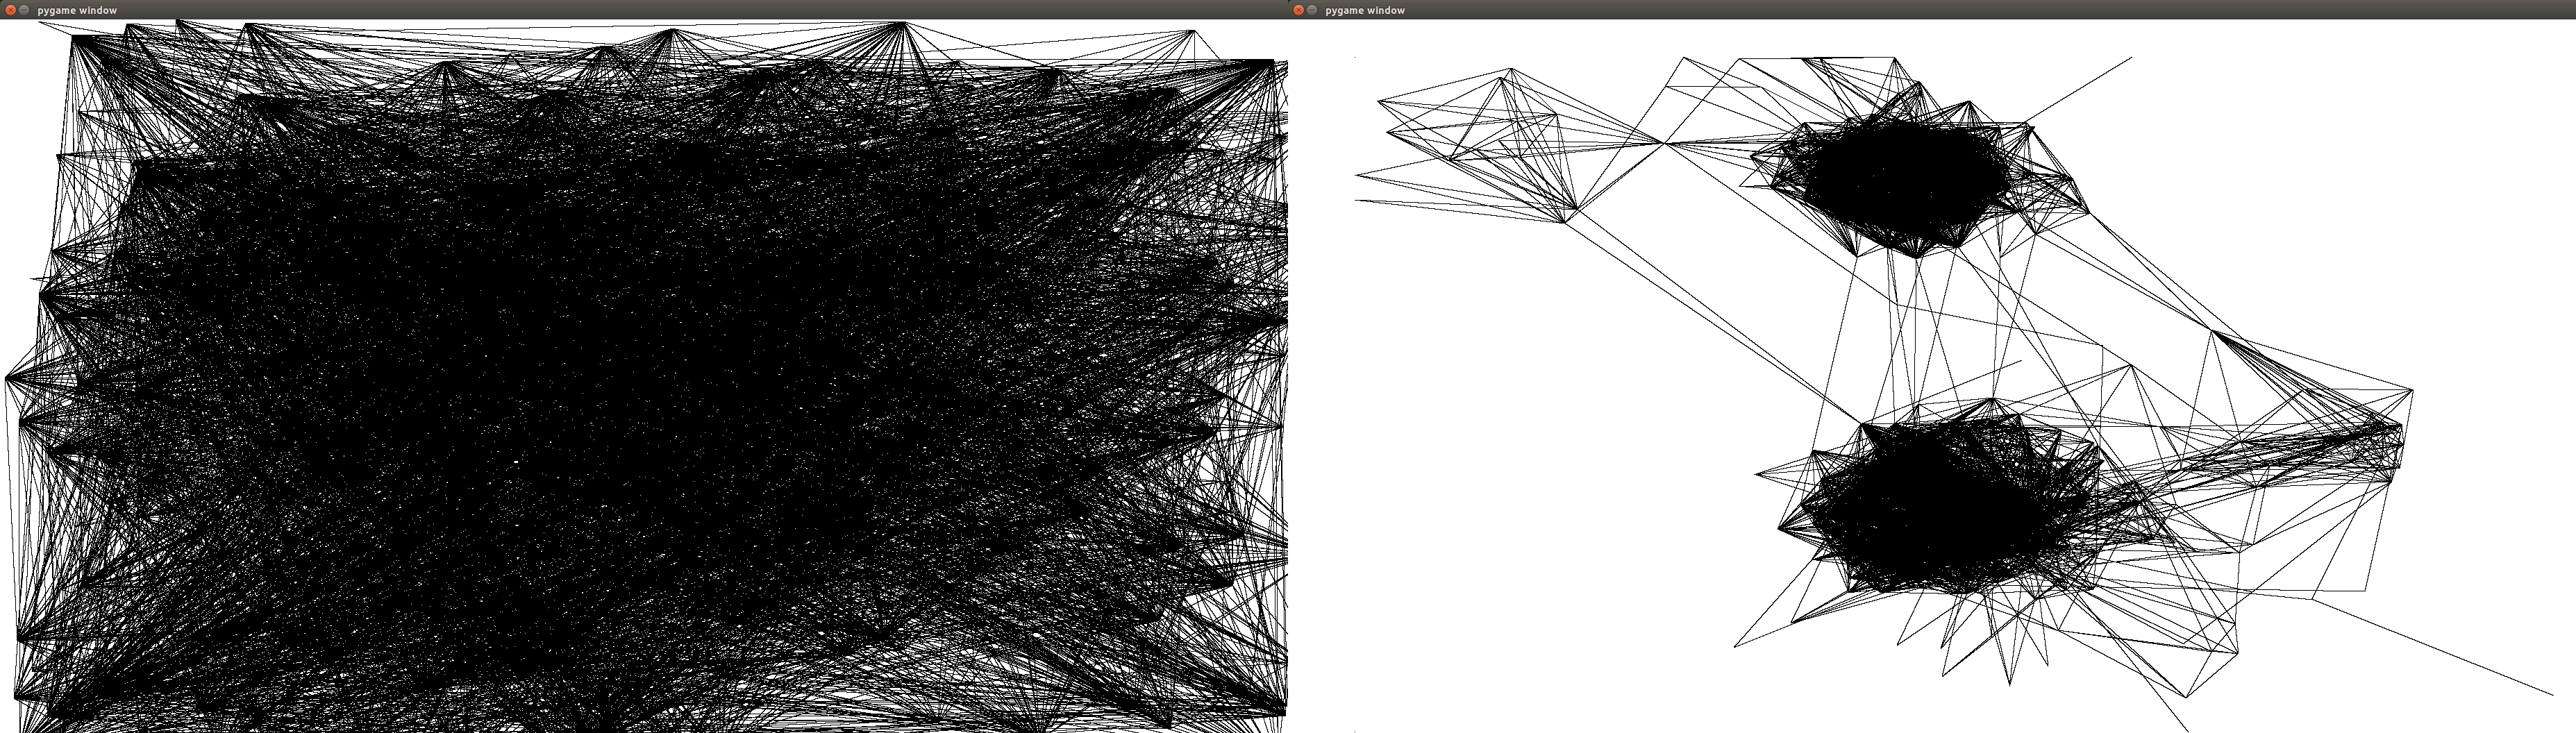
\includegraphics[scale=0.12]{Pygame.png}
\end{figure}

I have detailed the algorithm that I used in Algorithm \ref{alg:graph}. This is split into three main parts after the set up. where the value of $k$ is set to the value suggested in the above paper and $t$ is set to a value which was determined through experimental testing to be the best.

Ever vertex starts with 0 displacement. The first part of the algorithm then calculates the repulsion between every pair of vertices and updates its displacement an amount proportional to the inverse of the distance. The second part of the algorithm then calculates the attraction along every edge and updates the displacement of each vertices in this edge proportionally to the square of the distance. Finally, each vertex is moved either its displacement or t, a pre-determined distance, whichever is smaller, then the algorithm checks that none of the points have been moved outside the boundary of the screen.

In my implementation, the input graph is initially laid out totally at random. We can then see an example of an application of this algorithm over a number of iterations in figure \ref{fig:layout}. It can be seen how the points are taken from a random layout to a layout in which it is easy to see the structure of the graph.

\subsection{Lens}

Many of smaller details of graphs, especially when they include a large number of nodes can become hidden. After experimentation it was decided that a Gaussian lens would be best suited for this. This allows a gentle falloff and smooth transition through the point of maximum magnification that made the interaction natural as the user moved the 'lens' around the visualisation. Gauss's equation is given by 

\begin{equation}
\label{eq:Guass}
f(x,\mu,\sigma)=\frac{1}{\sigma\sqrt{2\pi}}e^{\frac{(x-\mu)^{2}}{2\sigma^{2}}}.
\end{equation}

In my solution $f(x, \mu, \sigma)$ represents the distance that the point will be displaced away form the cursor. In my implementation $x-\mu$ is the initial distance between the vertex and the cursor and $\sigma$ is a value that was determined by experiment in order to give the best result. I settled on 0.1, meaning that vertices over 20\% of the width or height of the screen away would no longer be significantly affected.

\begin{figure}[htb]
\caption{Example of lens}
\label{fig:lens}
\centering
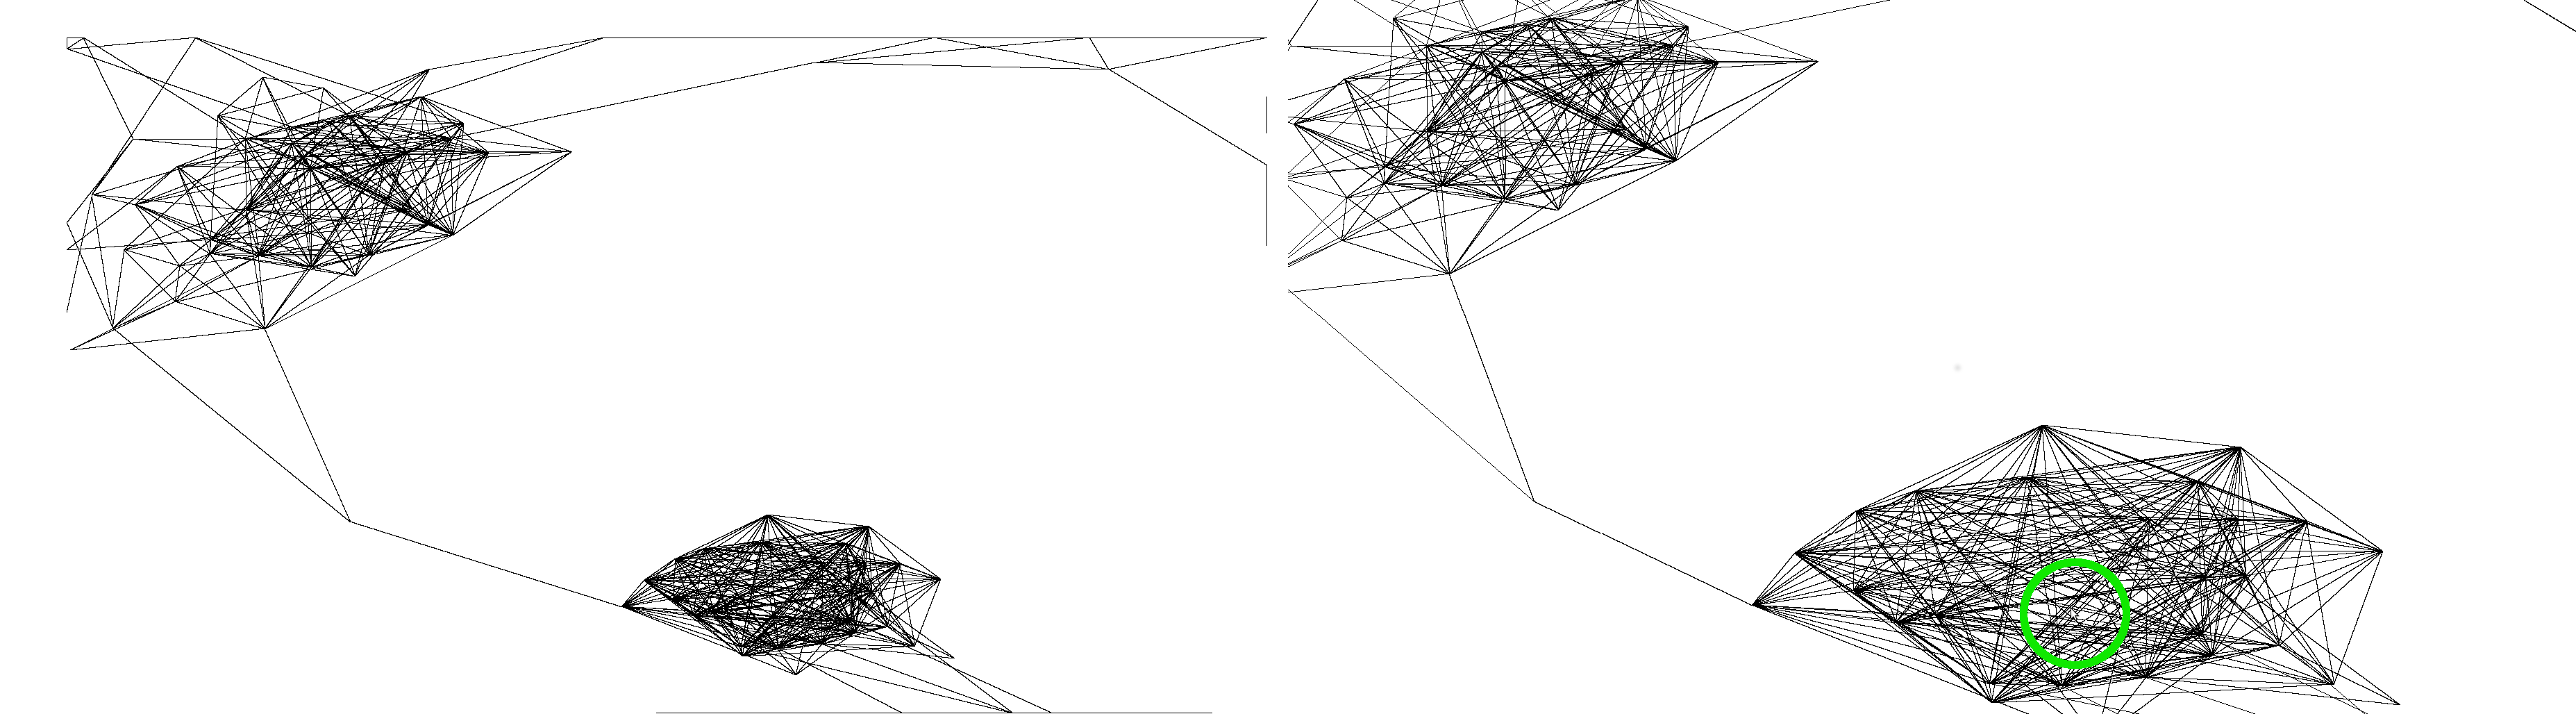
\includegraphics[scale=0.12]{Gaussian.png}
\end{figure}

It can be seen in figure \ref{fig:lens} that the lens allows the interactions surrounding the cursor (highlighted by a green ring) to be viewed much more effectively.

\subsection{Transitions}

One way of showing interactions between users in real times is by showing movement in the graph. An example of this can be seen in figure \ref{fig:transitions}. In this example these might be used to show 'likes'. As a user likes another's post a Facebook 'thumb' image is generated at the person who likes and travels over the course of about a second to the person who's post is being liked.

It is possible to use this as well to represent other interactions such as the spread of influence. The 'thumb' can be replaced by another image or by a simple disc or other relevant symbol.

\begin{figure}[htb]
\caption{Examples of transitions}
\label{fig:transitions}
\centering
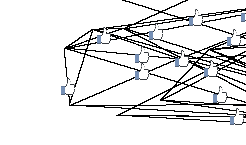
\includegraphics[scale=1]{Transitions.png}
\end{figure}

\subsection{History}

In order to make a fast moving interaction more clear, it is possible for the system to record the state of each user at given times and then to display this data once the model has run.

\begin{figure}[htb]
\caption{Example if a display of the history of states}
\label{fig:history}
\centering
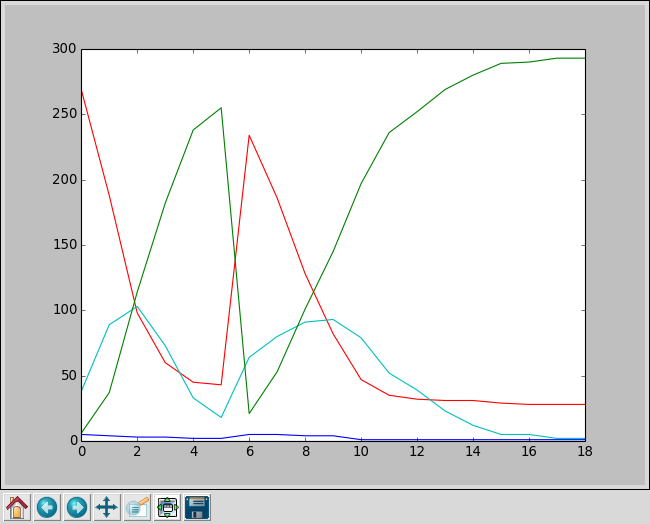
\includegraphics[scale=0.3]{Graph.png}
\end{figure}

An example of this can be seen in figure \ref{fig:history}. The horizontal axis represents time while the vertical axis represents the number of users. In this case the colours in the graph match the colours that are used to represent the vertices in the graph view.

This visualisation makes it clear how the distribution of users changed over time. In this view the progress of the first campaign can clearly be seen, as can the jump when this campaign is ended and a second introduced.

\subsection{Vertices}

The system allows for many different ways of representing people as vertices depending on their attributes in order to make it as clear as possible what is being represented.

\begin{figure}[htb]
\caption{Examples of possible representations of vertices}
\label{fig:vertices}
\centering
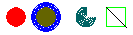
\includegraphics[scale=1]{Nodes.png}
\end{figure}

Figure \ref{fig:vertices} shows examples of different ways that attributes of the vertex can be changed in order to show different information.

The vertex on the left represents the most basic at only one solid colour, this colour could change for example to represent changes of state between a finite number of states or could have its brightness or hue changed to represent a continuous change in a property.
%For example in the advertising system detailed below the vertex changes colour to indicate what stage it has reached in the viral campaign.

The second vertex from the left shows that this can be build up in layers with an edge or another band of colour. This could be used to represent multiple properties win the same vertex.
%For example if the user wanted to track the difference that starting variables made to a system or to run multiple systems simultaneously that all relied on being represented by colour change of the vertex.

The second vertex from the right shows how it is then further possible to represent properties by the length of a filled arc around a vertex. This could be used to represent the state of a property that it is known will fall between two bounds for example age.

The final example on the far fight shows how it is possible to represent vertices as arbitrary shapes constructed as necessary in order to be fully customisable for whatever is being represented at the time.

\subsection{Edges}

There are multiple ways of using edges of the graphs to represent the relationships between people. A selection of these can be seen in figure \ref{fig:edges}.

\begin{figure}[htb]
\caption{Examples of possible representations of edges}
\label{fig:edges}
\centering
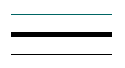
\includegraphics[scale=1]{Edges.png}
\end{figure}

The bottom line shows how edges are generally represented as a single pixel line joining the two users who have a relationship between then.

The middle like then shows that the thickness of the line can be changed in represent different things about the relationship between two people. This could for example be used to represent the strength of the relationship between two people.

On the right I have shown how it is possible to change the colour of the line joining the two vertices. This could be changed to represent some interaction between he users and can obviously be combined with either of the two previous methods.

Finally it is also possible to add significance to the weight of the lines by adjusting the graph layout algorithm. This could then be used to affect the shape of the graph so that, for example, users who interacted more frequently were more clustered.

\subsection{Demonstration Models}

In my implementation I included a set of demonstrations in order to show off the usefulness and effectiveness of my implementation as applied to real-world scenarios.

\subsubsection{Influence}

I implemented the two models of influence spreading through a social network according to \cite{kempe2003maximizing}. This could be used to model behaviour adoption across a social network, for example if a new social game such as 'Farmville' were to be released, this could simulate how social network users would encourage their friends to also play the game.

In the first model of influence, based on 'Linear Threshold Model', initially each vertex is given an adopted value of $False$ a value representing the influence that they are currently feeling and an adoption value, representing how much influence must be exerted over them in order for them to adopt the behaviour. A given set of starting nodes are then chosen and have their adopted value set to $True$. The model then proceeds in steps. At each step, first the weights of all connections to that vertex are added up, then the weights of each vertex that has adopted the behaviour. If the weights of vertices that has adopted divided by the weights of all neighbour is greater than the vertices adoption value, that vertex then adopts the behaviour.

In the second model of influence based on the 'Independent Cascade Model'. Initially, similarly to before each vertex is given a property to show that it hasn't adopted the behaviour, and a random set are chosen to have adopted it. As before the model then proceeds in steps. In each step, each vertex that has adopted the behaviour will have one chance to influence its neighbours to adopt the behaviour. Whether or not they are successful depends both on the 'strength' of the edge between the two vertices and a random element. Each node that is successfully influenced has only one chance to influence its neighbours, but one node will have multiple chances to be influenced if it has multiple neighbours who are influenced.

In this model it is possible to configure many different aspects such as the number of starting nodes and the relative chances of the behaviour being adopted. It is also possible to use both models simultaneously in order to compare their results.

\subsubsection{Advertising}

A model of the spread of viral advertising was implemented based on a pre-existing method \cite{van2010viral} which relies on a transition of each person between a number of states. These states are: People who haven't participated in the campaign; people who have received a 'seed' email; people who have seen a traditional advert as part of the campaign;  people who have received an email from a friend about the campaign; people who have chosen not to participate and finally people who have participated.

In the initial set-up, all vertices have a status set that they have not participated in the campaign. A random number of 'seed' emails are then sent to people, then a number of 'seed' adverts are shown to the vertices, both with a chance to trigger participation in the campaign. As before this campaign proceeds in steps. At each step, a certain number of vertices being considered will check their email. If they have received an email related to the campaign, either from another user or a 'seed' email then this will give them either a chance to participate in the campaign or choose not to. If they choose to participate in the campaign, they will then generate emails to a random number of their friends about the campaign and the cycle continues.

In this case it is possible to change all of the relevant variables in order to see their effects such as the number of seed emails sent and the number of users initially seeing the seed advert. It is also possible to determine how likely a user is to respond to either an advert or an email or even to give different response rates for emails from their friends and seed emails.

\subsubsection{Recommendation}

I implemented a model such as might be found in a social recommendation system as inspired by \cite{walter2008model}. This model imagines a system in which users are recommended something, say, films according to what their friends report they enjoyed.

This system begins by seeding a number of ratings for a number of different items, ratings are a value between 0 and 1. Recommendations are then propagated through the graph. This happens once, each vertex looks through its neighbours to see if it can find someone who has a direct opinion of the product, if it fails to find anyone it then looks through its neighbours neighbours and so on until it either finds someone or reaches a pre-determined depth. If it does find somebody it then takes this recommendation with a degradation depending on how many edges separate the vertex under consideration and the one doing the recommending.

It is possible in this model to change several variables within the system such as the number of users that are initially seeded with experiences of what is being recommended, what experience these users have and the depth to which a user will search for a recommendation. This system also accommodates there being multiple items which can each have their own recommendations propagated independently.

%\subsubsection{Social}

%Finally I took a different approach and implemented a system of interactions such as might happen over a social network. For this I primarily used my personal experiences on Facebook, a platform that I use to interact with people online daily. It is difficult to find reliable statics to use in such a model but in the end I settled on a website which had correlated statistics from many sources of varying reliability \cite{facebookStats}. I was satisfied with this however as it was not necessary for my model to be perfect, only sufficiently accurate to show how my visualisation could be applied to a real situation.

%The model encompasses various elements of the Facebook website. Each user has a wall on which they can post either a status of a picture at random intervals, pictures can have one or more friends tagged in them. Each user also has an attribute 'views'. Users will at random intervals check their news feed which is made up of posts from the walls of their friends. Their attitude towards their friends can change according to their attitude towards any other people that might appear tagged in pictures, or the difference in 'views' between a person reading a status and the person writing it.

\subsection{Tools Used}

The solution is entirely written using a combination of Python 3.4 and various libraries. I used a 64 bit binary of version 3.4.2 of CPython as my interpreter, downloaded from www.python.org. This was chosen as at the time of writing it was the latest version of the most popular Python interpreter. I used a 64 bit edition so that if it became necessary I would be able to make use of all available memory of my computer and python 3 was chosen rather than python 2 so that I was able to make use of recent performance optimisations.

Visualisations were produced using the PyGame library. I obtained this by building the source available from https://bitbucket.org/pygame/pygame on my system at the time of writing with CPython as mentioned above. PyGame was chosen because if its ease of use over OpenGL allowing for rapid prototyping. Additionally its use of optimised C code would ensure that the visualisations would not interfere with time required for other computations.

Menus were implemented in the solution using the Python package Tkinter. This was obtained from my system's package repository (http://archive.ubuntu.com/ubuntu/dists/utopic/). I chose to use this as it would provide easy implementation of menus in my solution while not distracting from the models being used.

Graph drawing was done using the pyplot library from Matplotlib. This was as with Tkinter obtained from by systems package repository. I chose this as a method of graph drawing as it provided easy drawing of simple graphs and would easily allow me to change the style in order to experiment with different ways of displaying the data.

\subsection{Verification and Validation}

Software verification was undertaken at all stages of the implementation. This was primarily achieved with reference to my Design Report, in which I had given thought to the design and architecture necessary in order to achieve the objectives set out at the beginning of the project.

Software validation was made in reference to the objectives and functional requirements set out in my Design Report which were designed to allow me to meet the objectives of the project in several layered steps. This was also helped by the project supervisor who advised on direction at all stages and ensured that focus was maintained on the areas in which it was most needed.

\subsection{Testing}

As I prototyped my implementation, testing was mainly undertaken through a dynamic approach, matching the output given by the code to an expected output based on the software design. This was done at all stages of implementation in order to check progress against aims and ensure that subsequent work would be able to function on top of old as expected. In the case of algorithm checking however static testing was undertaken in order to ensure that the results that they gave were as expected.

The dynamic testing used a grey-box approach with a focus on the user output but with hopes of testing cases that would challenge the internal models driving the output.

While the system is highly modular, the modules all rely on one another in order to provide a useful output. Given that each module was fairly simple testing focused on an integration and system level enabling a focus to be given to the output visible to the user as was the focus of the project.

\subsection{Implementation Difficulties}

The main difficulty that I faced during implementation was the speed at which the Python would run using the interpreter on my computer. It was necessary at all times to make a special effort to ensure that algorithms remained as fast as possible so that the user interface would not spend long periods unresponsive as this would degraded the user experience so important to the project.

I attempted to rectify this by using an alternative Python interpreter PyPy. However, this did not support the Pygame binaries I was using at the time and I was unable to use it to build suitable binaries. While there is an alternative to Pygame compatible with PyPy, Pygame\_cffi (https://github.com/CTPUG/pygame\_cffi), at the time of writing this did not appear sufficiently complete or stable for use with the project.

Additionally, part way though the project, Facebook changed its privacy polity restricting the amount of data that was accessible through its API. This means that at the time of writing NetVizz is no longer able to download new data. It would be necessary therefore that an alternative solution was found in order to continue using a users's own social network data.

\section{Results}

In order to demonstrate my system I made several mock ups to show what it could be capable of. I present those here.

\subsection{Viral System}

Here I implemented the viral advertising model specified above. I will then use this to demonstrate various aspects of the representation possible in my system.

\begin{figure}[htb]
\centering
\captionsetup[subfigure]{justification=centering}
	\begin{subfigure}[b]{0.3\linewidth}
	\caption{Viral graph view, showing the states of the people}
	\label{fig:viralStates}
	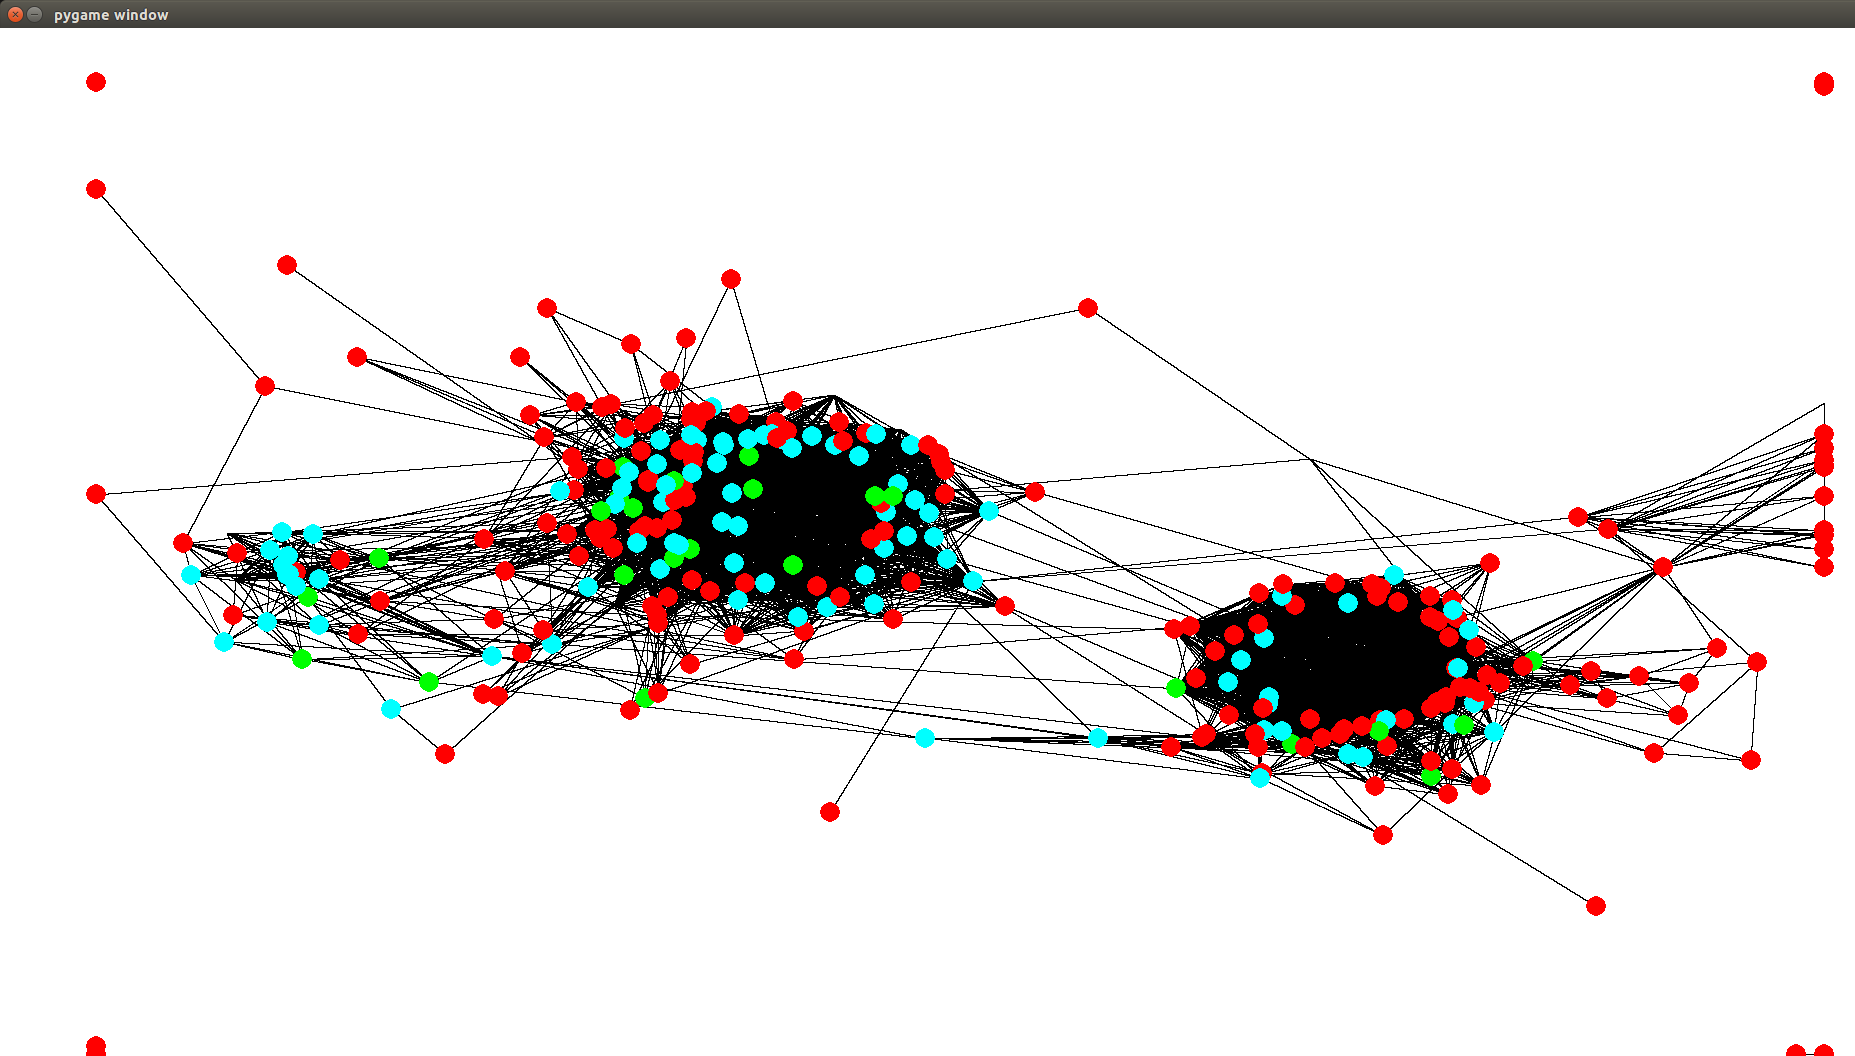
\includegraphics[scale=0.1]{Viral1.png}
	\end{subfigure}
\\
	\begin{subfigure}[b]{0.3\linewidth}
	\caption{Window showing configuration of new viral campaign}
	\label{fig:viralConfig}
	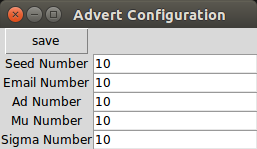
\includegraphics[scale=0.3]{Viral2.png}
	\end{subfigure}
\quad
	\begin{subfigure}[b]{0.3\linewidth}
	\caption{Graph showing evolution of states of people over time}
	\label{fig:viralGraph}
	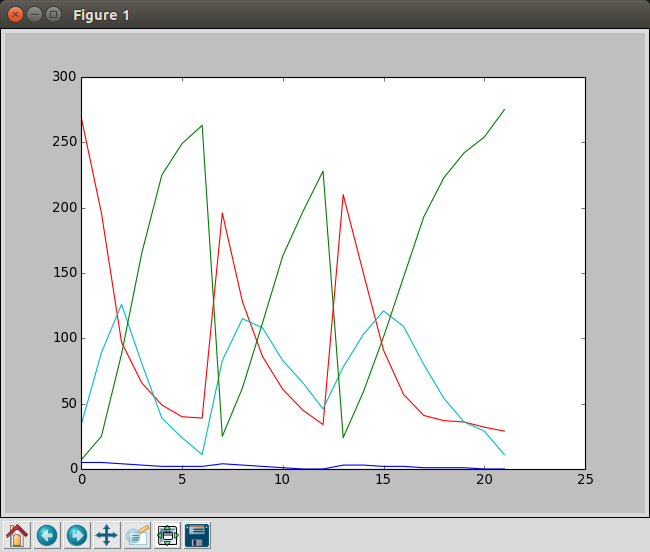
\includegraphics[scale=0.2]{Viral3.png}
	\end{subfigure}
\caption{Examples of output produced from Viral model}
\label{fig:viral}
\end{figure}

In figure \ref{fig:viralStates} we can see a representation of the state of all the actors involved in the model. In this case the colour represents the current state of the person in relation to the current campaign. It can immediately be seen that people at the edge of the network haven't yet heard about the campaign at all and are in red, meanwhile the people who have already been sent emails (in turquoise), can clearly be seen to be clustered around the people who have already taken part in the campaign (in green).

Figure \ref{fig:viralConfig} clearly shows the kind of configuration that is possible when adding a new campaign during the running of the model along with a set of preset suggested parameters.

Figure \ref{fig:viralGraph} demonstrates how the time evolution of the model can then be shown after it has run. On the vertical axis we have the number of people in each state at a given time and on the horizontal axis we have the number of iterations of the simulation. The colours match those that were used to represent the states on the graph. This clearly allows features to be picked out such as the beginning of new campaigns as well as more subtle features such as the time it takes for people who haven't yet participated to outnumber those who have.

\subsection{Recommendation System}

The same can be seen with the recommendation system which demonstrates a different set of features.

\begin{figure}[htb]
\centering
\captionsetup[subfigure]{justification=centering}
	\begin{subfigure}[b]{0.4\linewidth}
	\caption{Initial graph view showing who has experienced and who has been recommended a product}
	\label{fig:recommendationInitial}
	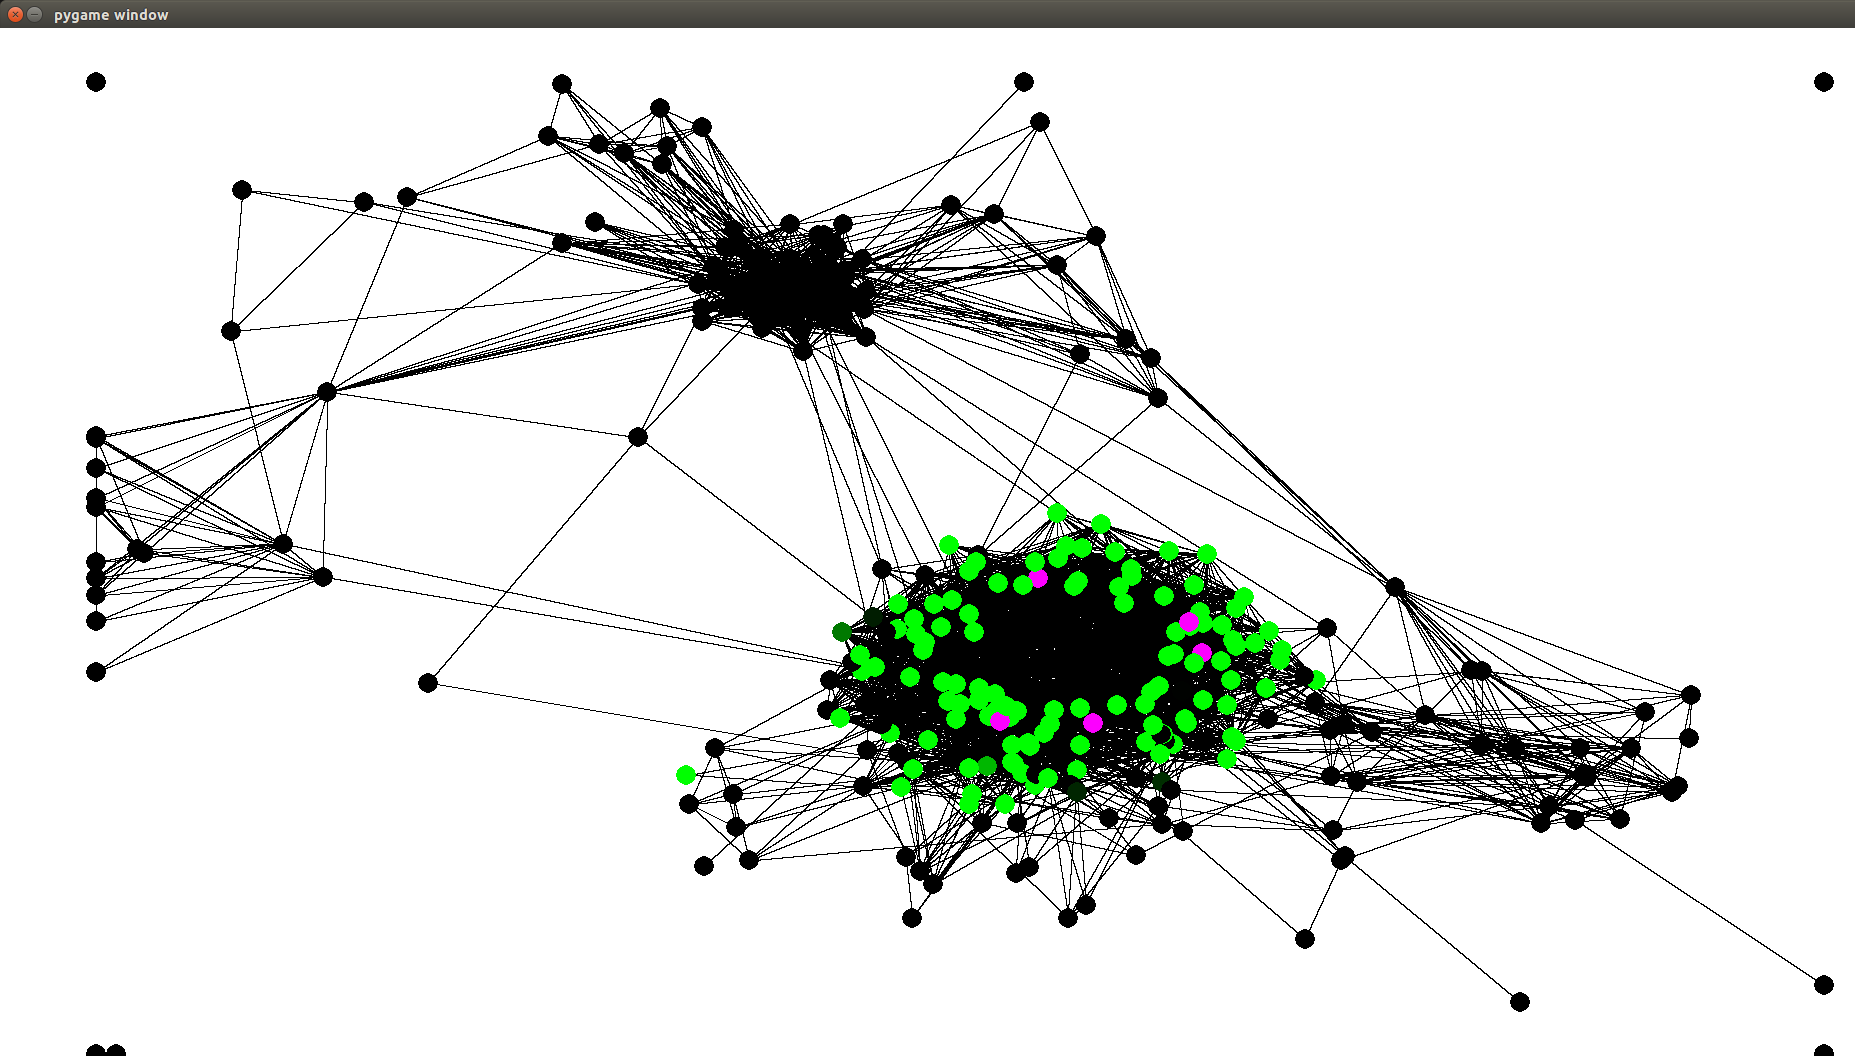
\includegraphics[scale=0.1]{Recommendation1.png}
	\end{subfigure}
\quad
	\begin{subfigure}[b]{0.4\linewidth}
	\caption{View demonstrating everyone's favourite product}
	\label{fig:recommendationFavourite}
	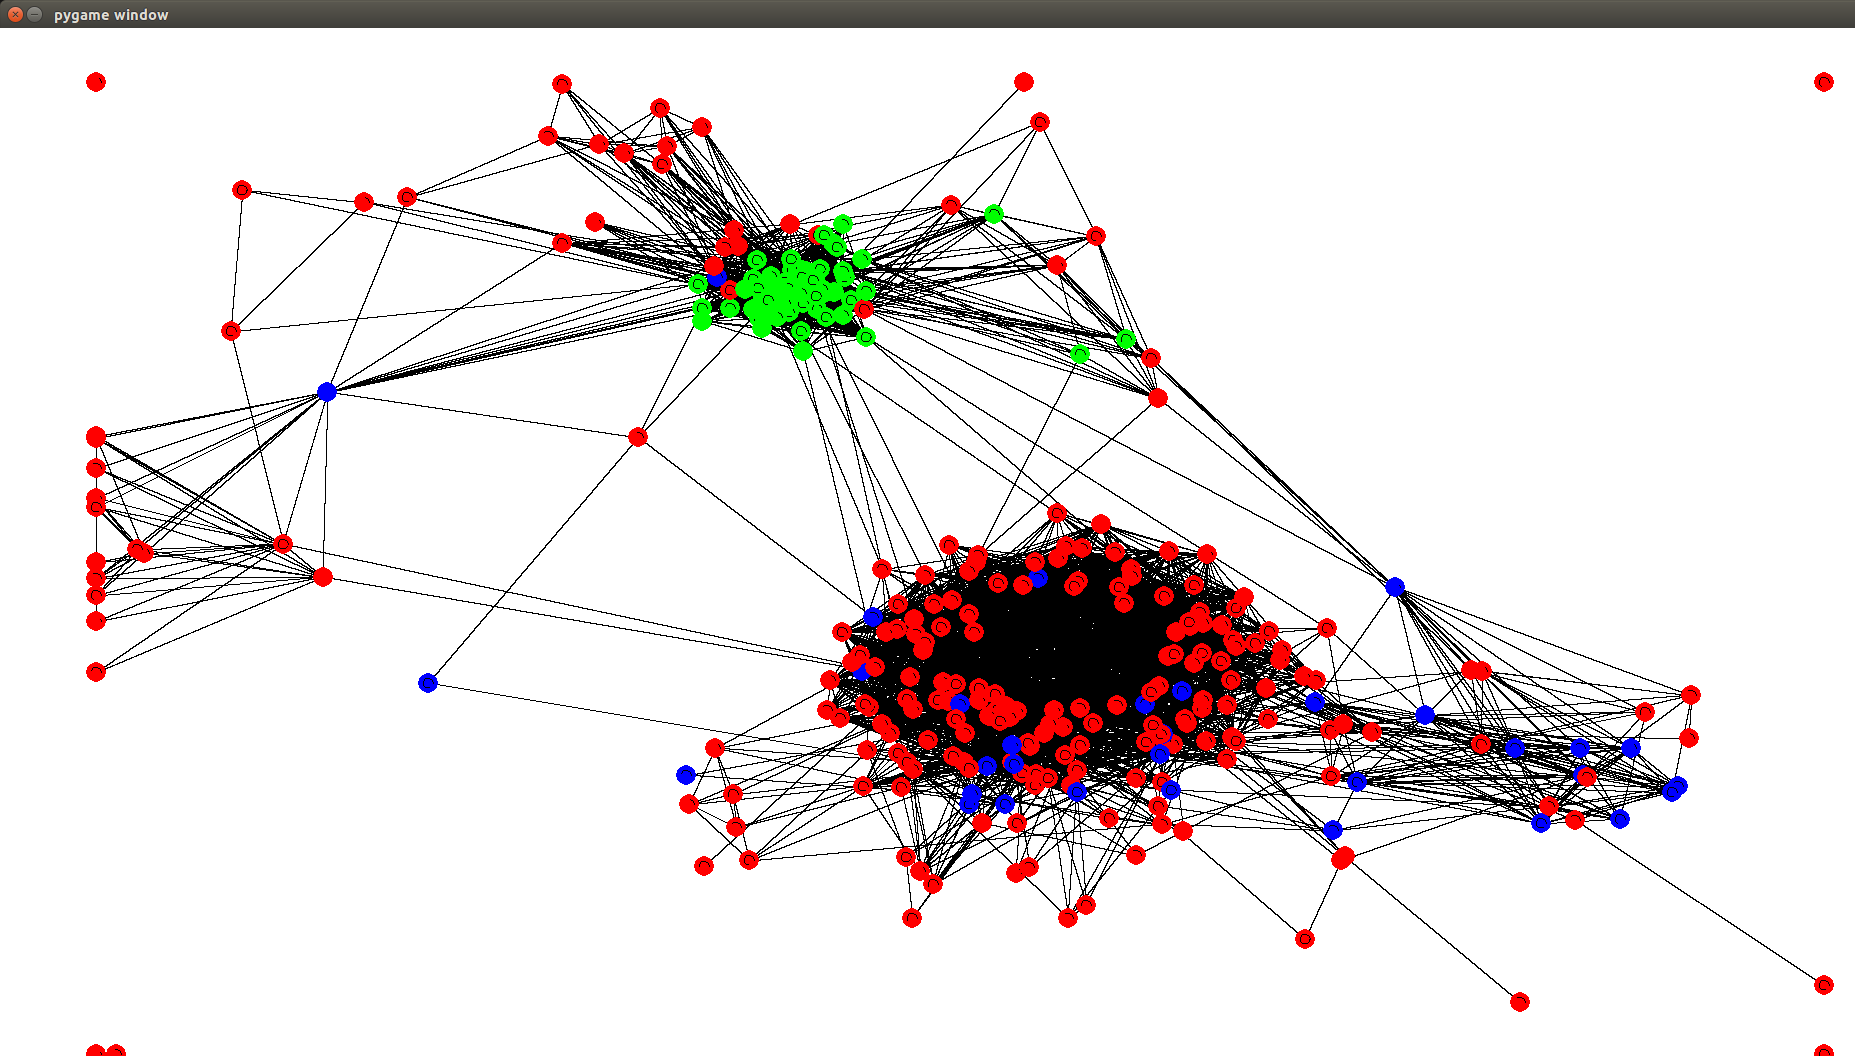
\includegraphics[scale=0.1]{Recommendation2.png}
	\end{subfigure}
\\	
	\begin{subfigure}[b]{0.4\linewidth}
	\caption{View comparing what products people like}
	\label{fig:recommendationComparison}
	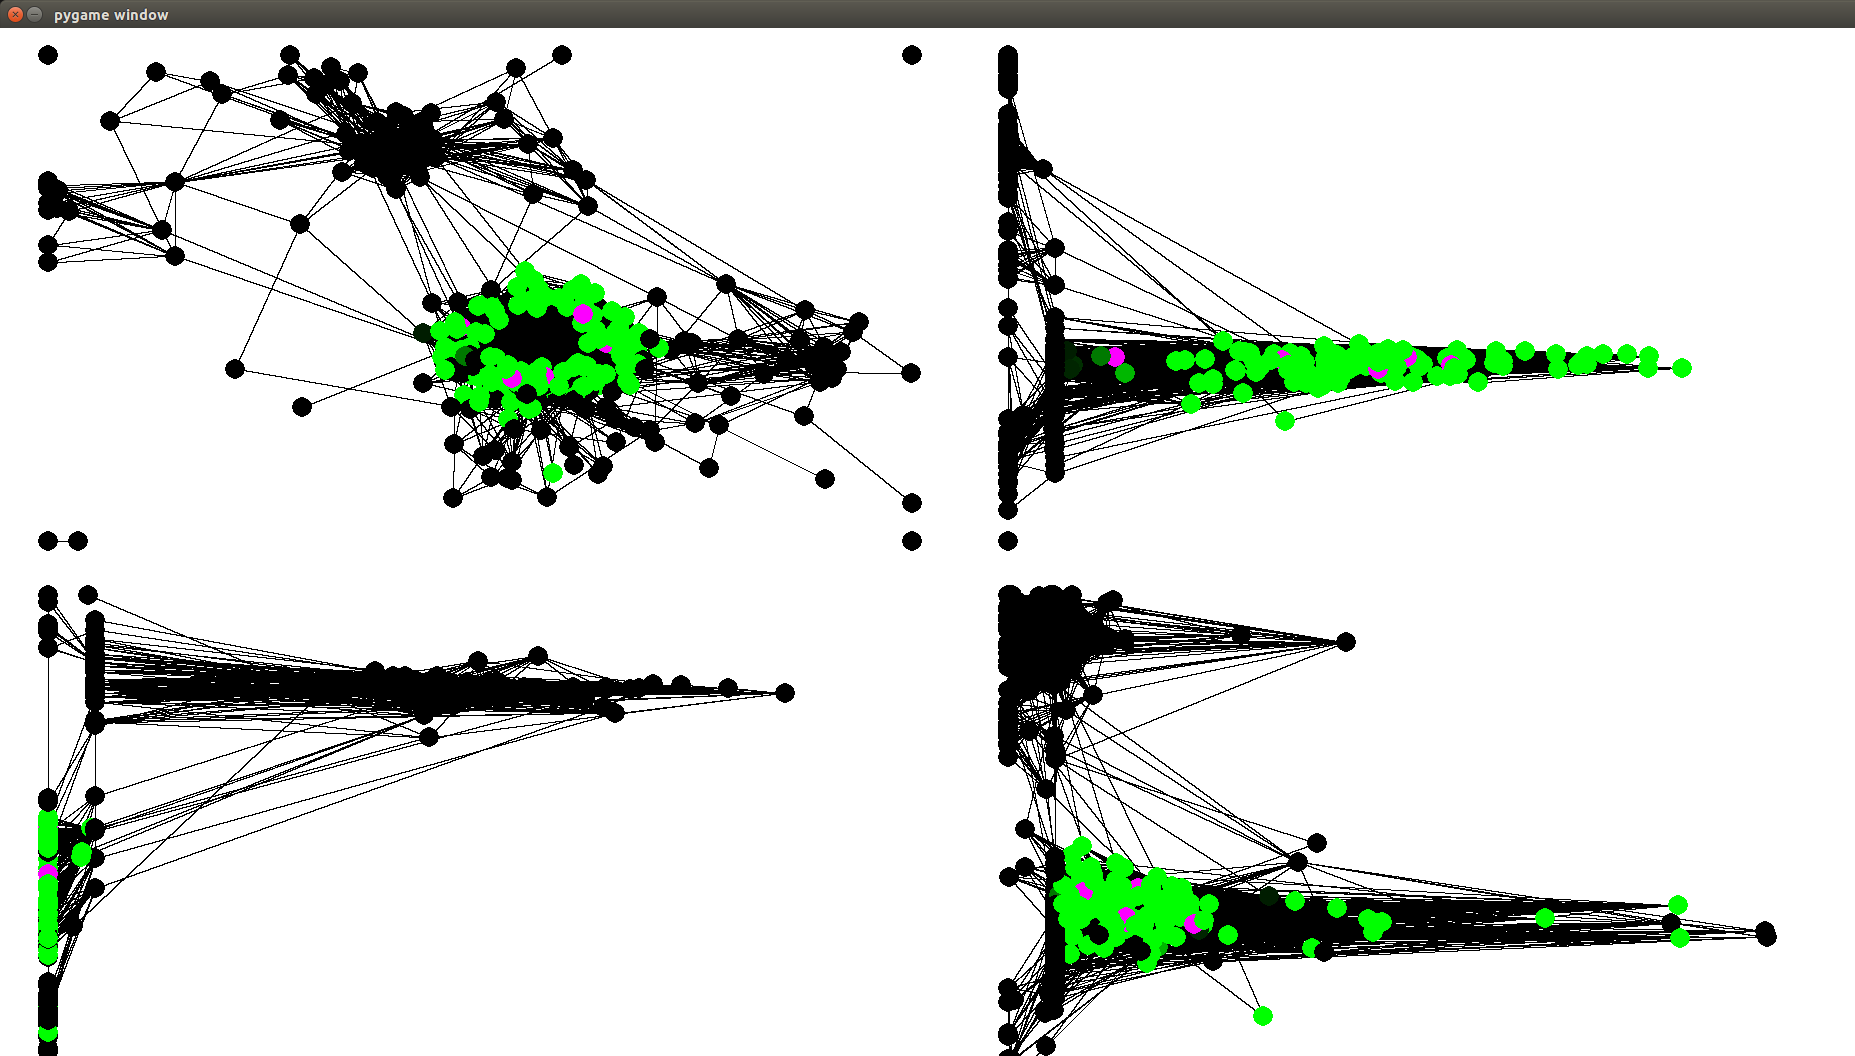
\includegraphics[scale=0.1]{Recommendation3.png}
	\end{subfigure}
\quad
	\begin{subfigure}[b]{0.4\linewidth}
	\caption{View showing different distribution of preerence for another product}
	\label{fig:recommendationDifferent}
	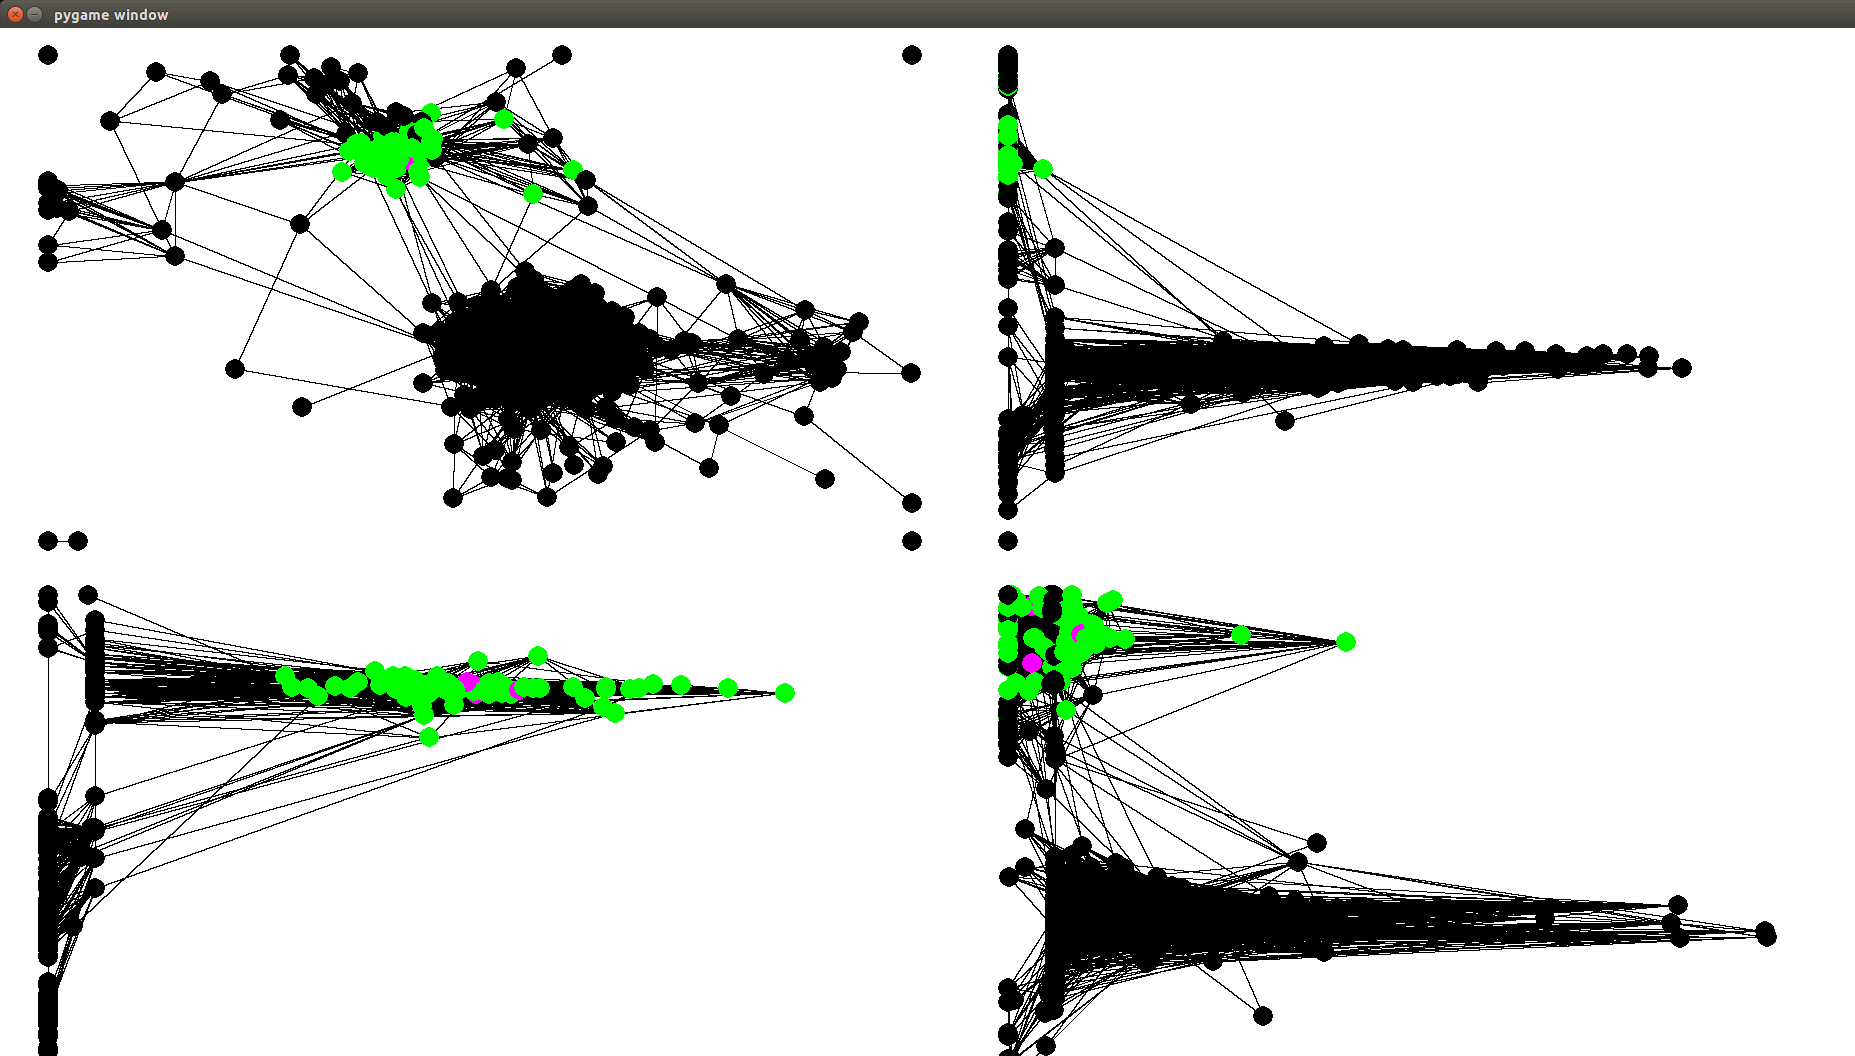
\includegraphics[scale=0.1]{Recommendation4.png}
	\end{subfigure}
\caption{Examples of output produced from the recommendation model}
\label{fig:recommendation}
\end{figure}

Here we can see in figure \ref{fig:recommendationInitial} that the user is able to see the effect of those who have experience of a product on who will be recommended it. In this case those people who appear purple have a direcct experience meanwhile those who appear in green are those who will be recommended the product. The brightness of the green depends on the confidence of the recommendation.

Figure \ref{fig:recommendationFavourite} then demonstrates a different way of looking at this data. The colours represent the item which each person is most likely to enjoy.

Then in figure \ref{fig:recommendationComparison} we can see a different layout of the data. Here each of the streched horizontal polts represents one of the products while the horizontal distance to the right represents how much they are likely to enjoy the product. The comparison between this and figure \ref{fig:recommendationDifferent} then shows the interaction between the way different people enjoy different products and the extent to which enjoyment of one product will mean that they enjoy another

\subsection{Influence}

Finally I did the same with the influence system detailed above.

\begin{figure}[htb]
\centering
\captionsetup[subfigure]{justification=centering}
	\begin{subfigure}[b]{0.4\linewidth}
	\caption{Showing selection of vertices to be influenced}
	\label{fig:influenceSelect}
	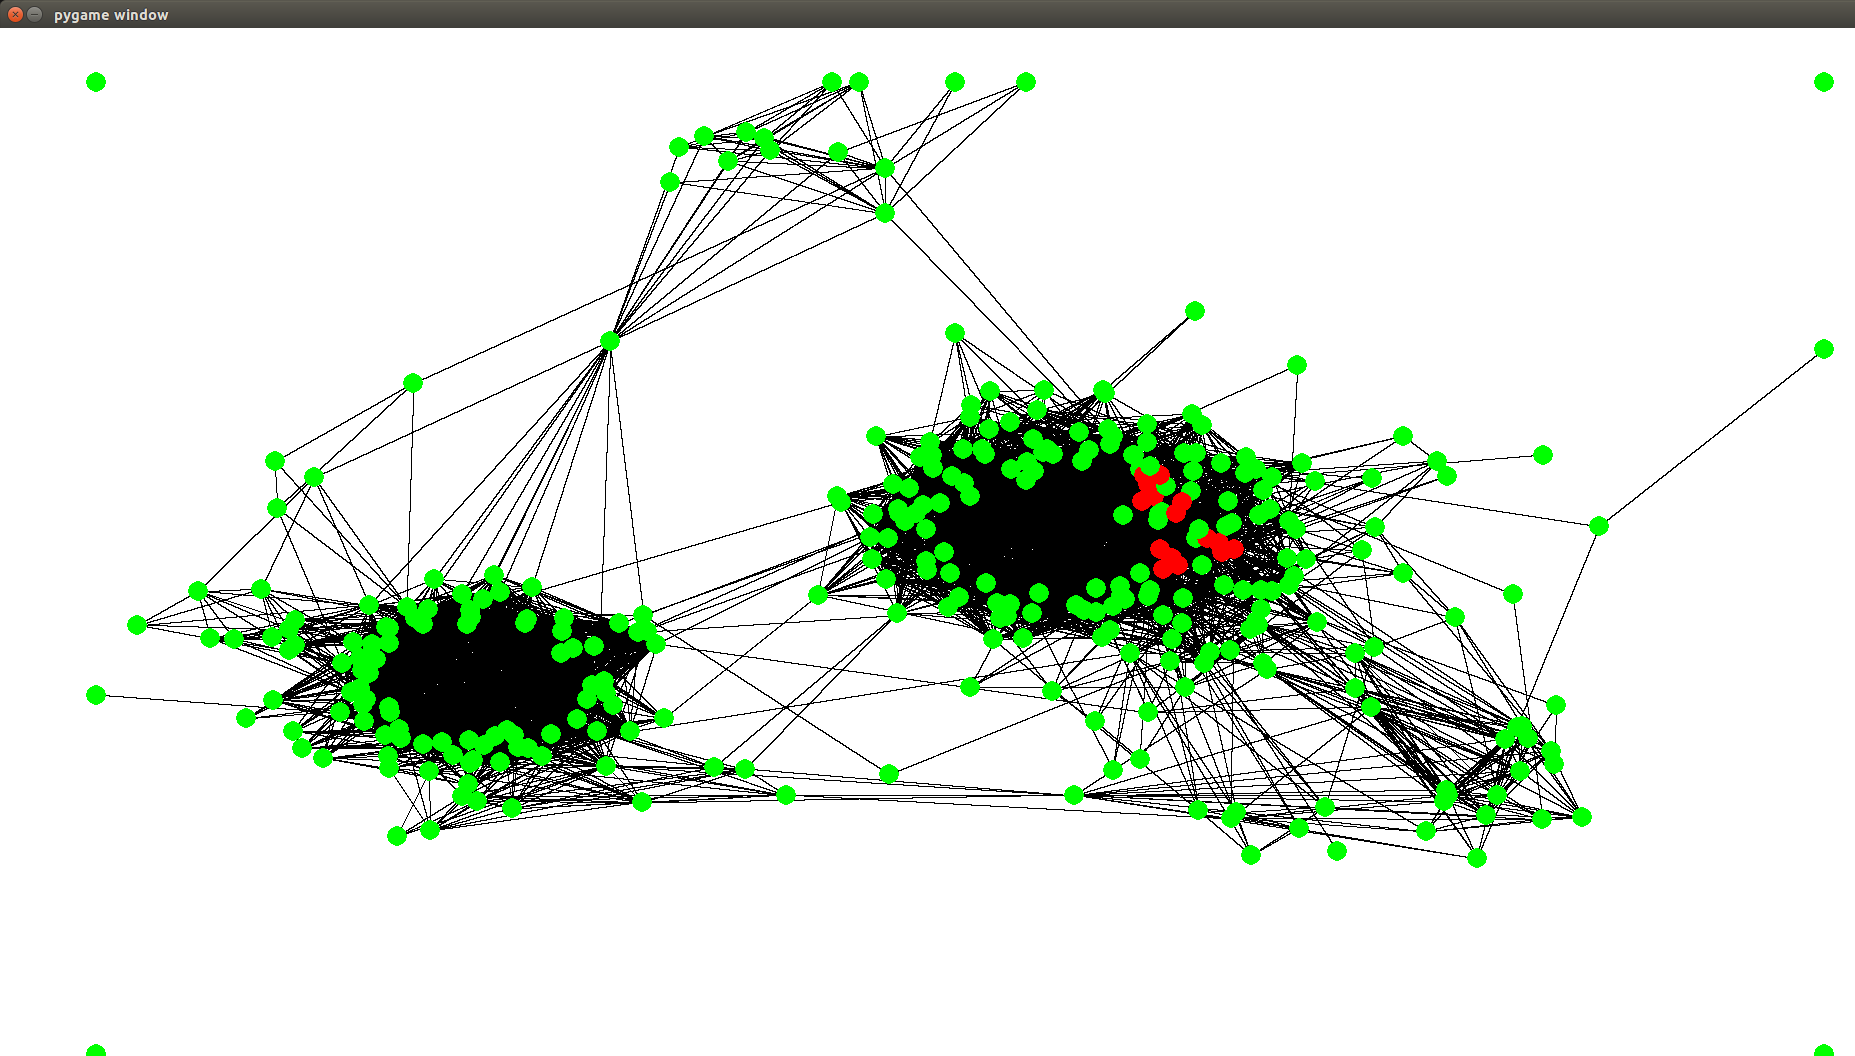
\includegraphics[scale=0.1]{Influence1.png}
	\end{subfigure}
\quad
	\begin{subfigure}[b]{0.4\linewidth}
	\caption{Showing comparison of two models of influence spread}
	\label{fig:influenceCompare}
	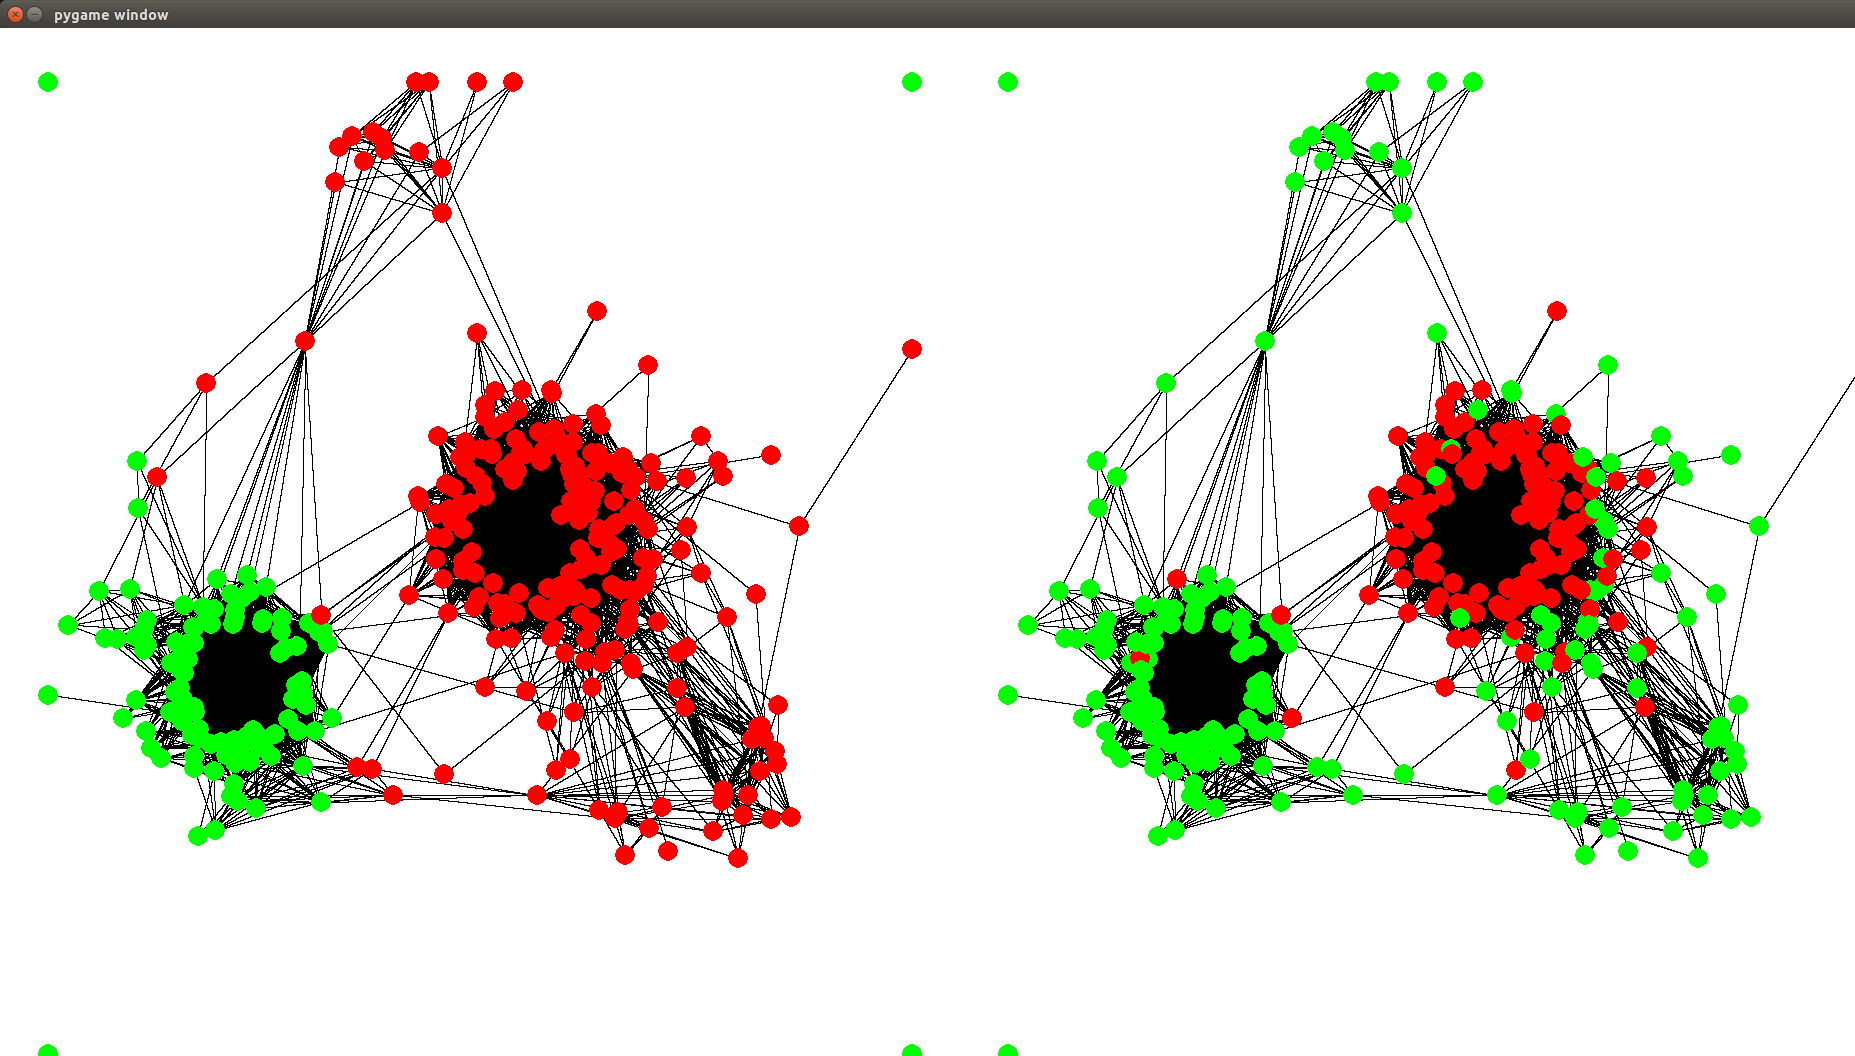
\includegraphics[scale=0.1]{Influence3.png}
	\end{subfigure}
\caption{Example outputs form the influence package}
\label{fig:influence}
\end{figure}

In figure \ref{fig:influenceSelect} we can see the operation of the user selecting which will be the people who are initially responsible for influencing the rest of the population. This selection occurs by clicking on the green circles which then turn red to indicate they have been selected.

We can then see in figure \ref{fig:influenceCompare} how it is possible to compare the two different models of the spread of influence. Once a person has become influenced they turn from green to red allowing the differences in the models to be seen in real time.

\section{Evaluation}

I will evaluate my project according to Edward Tufte's principles of information visualisation \cite{tufte1983visual}. These represent a check-list for effective data visualisation that, although it is many years old is still often used in connection with modern graphic design.

Therefore according to Tufte, graphical representations should:

\begin{enumerate}
\item {\bf Show the data}

I believe it is clear that my system does indeed show the data. This item is included to ensure that actual data is being shown rather than simply results of computation or some other qualitative measure.

\item {\bf Induce the viewer to think about the substance rather than about methodology, graphic design, the technology of graphic production or something else}

My solution is to some extent able to allow the viewer to focus only on the substance than the  implementation as it is able to 

\item {\bf Avoid distorting what the data has to say}

Some aspects of my system ensure that the data is not distorted, for example where a property is represented by something that can have an absolute relationship to a feature of the graph like colour this makes it impossible for the system to distort data. On the other hand in elements like the layout where an iterative algorithm is used to layout with results that are difficult to predict before, this leave the possibility of distortion if the layout algorithm were to find an poor local minimum. 

\item {\bf Present many numbers in a small space}

My solution can take up any pre-defined area, by default it produces an output the size of the whole screen. However, my solution also tries to ensure that in order to show the maximum amount of data it can it does this in an efficient way. However, my solution is optimised for certain scales rather than being able to accommodate a wide range of display sizes.

\item {\bf Make large data sets coherent}

This isn't something that my system is able to do. Due to the nature of the layout algorithm the system becomes unusably slow beyond a few hundered data points. Additionally, beyond this number the view will become too cluttered and make the visualisation unusable

\item {\bf Encourage the eye to compare different pieces of data}

The system ensures that it is possible for different pieces of data to be compared. It achieves this through a side-by-side comparison as can be seen in the figures \ref{fig:influenceCompare} and \ref{fig:recommendationComparison}. Figure \ref{fig:recommendationComparison} also shows an alternative way of comparison whereby different colours can be applied to the same points in order to show differences.

\item {\bf Reveal the data at several levels of detail, from a broad overview to the fine structure}

My solution doesn't perform particularly well at this aspect as it follows a broadly flat graph model. However, it integrates some aspects of this in its ability to view extra data through hovering over data points or using magnification of areas of the graph which are very tightly packed.

\item {\bf Serve a reasonably clear purpose: description, exploration, tabulation and decoration}

The extent to which my implementation fulfils this purpose depends on what it is applied to as it is designed that it could be applied to many different data sets. It can be seen for example in the influence application that each element has a clear description, however the exploration of different elements...

\item {\bf Be closely integrated with the statistical and verbal descriptions of the data set}

This is an element that my solution does not address particularly effectively. First of all it was not a part of the project to provide a verbal explanation of the data and in many cases the visualistions themselves have little meaning without such explanation. However, in some cases my visualisations are closely related to statisitical representations of the data set.
\end{enumerate}

%As detailed in the Design Report I will take two approaches to evaluation. First I will take 4 criteria and use them to compare my solution to three other, similar solutions, Gephi \cite{ICWSM09154}, Vizster \cite{heer2005vizster} and WolframAlpha Facebook report \cite{wolfram}. Then second I will look at the application of my solution to real-world problems in order to see if it offers anything additional to what was previously available.
%
%\subsection{Comparison}
%
%\begin{enumerate}
%	\item {\bf The ability of the system to clearly represent the state of and relationships between people}
%	
%	Compared to Gephi my implementation does a similar job of representing the states of people using the same methods such as changes in size and colour of the nodes of the graph. Gephi also represents relationships in the same way, using simple lines of connection.
%	
%	Vizster uses people's names to represent them rather than symbols, emphasising the importance of the actual people. However, it represents relationships in the same way using a series of lines however in this case I believe it works better than my implementation in the cases which Vister was intended for.
%	
%	WolframAlpha again uses colours and lines to represent people's relationships and so is very similar to mine.
%	
%	\item {\bf The ability of the system to represent the interactions over different modes between people}
%	
%	None of the other systems represent dynamic interactions, but only static relationships, in this respect my system is more effective than any of them.
%	
%	\item {\bf The ability of the system to represent clustering of the people in the system based on interactions}
%	
%	As none of the other systems represent interactions, but only the static relationships between people, my system is clearly the more effective in this respect. My system is able to visualise the clustering both in respect to the layout of the data and an output of qualitative data
%	
%	\item {\bf The ability of the system to output quantitative data which can be used to draw useful conclusions regarding the nature of some aspect of the evolution of the model over time}
%	
%	Gephi has a significant amount of numerical output, presented in the form of graphs, showing many aspects of clustering, however, this does not change over time. As a static view however it is superior to my solution.
%	
%	Vizster does not offer any numerical output.
%	
%	WolframAlpha does not immediately offer and numerical output, however it can be gained if the user then extracts the graph data so while my solution provides better initial data, with effort WolframAlpha can provide more insight.
%\end{enumerate}
%
%\subsection{Applications}
%
%\subsubsection{Influence}
%
%This system is slightly less well suited to a system of influence spread as this doesn't rely on such complex interactions between the users. However, it still remains useful in order to see a comparison between two instances of this mode, even if it isn't of interest itself. Even in this case my system provides significant improvement in a static system as, even though the interactions are simple, they evolve over time.
%
%\subsubsection{Advertising}
%
%I believe that this is a good application for this system. It is useful to be able to see the transition between various states and the system is particularly good at representing this state transition through the use of colour.
%
%Also the ability to then visualise these changes over time at the end means that even features of the system that would be missed by watching it in real time can be analysed later.
%
%\subsubsection{Recommendation}
%
%This is again a good application for this system as it is possible to see clustering that varies depending on the starting conditions for the system. It also allows important comparisons between multiple systems within itself. However this would be able to be represented as easily in a system showing static relationships as, when the recommendations are calculated the system then remains static.

\section{Conclusions}

I believed I have managed to some extent to produce a solution that was able to combine previous research in data presentation of social networks and apply this to a dynamic system of interactions. On top of this I think that my system is able to be applied to various scenarios which show its benefit.

I can demonstrate that I have built on previous research though my implementation of various of its features in the Solution section. This shows that it is indeed possible to use research previously done on static network and apply this to dynamic systems of interactions.

My results show that my system is not only able to extend previous work to include visualisation in new ways that were not commonplace before but that on top of this it is also able to handle similar visualisation to that currently exists simultaneously.

On top of this the 'models' that I have implemented show that this system is a useful one that can be applied to a diverse range of systems. The three that I have demonstrated here are all very different in nature but my system is able to offer some unique way of viewing each. I hope that these applications are also more useful that previous efforts to visualise them using a static system of relationships and that this allows for greater insight into their evolution.

In the future I believe that my work would benefit from re-writing in a faster language than Python which would provide two benefits. First it would allow more computation of the data to take place, particularly where data was changing in real time according to multiple models of evolution at once. Secondly it would allow a better user experience with smoother interactions as the program was no longer waiting between drawing each frame and updating the view.

Another potential extension my work would be to provide a more cohesive interface that allows the user to interact with models in more depth as they are being run. For example the user may wish to change the way in which something is represented and didn't want to start the system again with new settings.

\bibliography{projectpaper}


\end{document}